\documentclass[10pt]{report}

\usepackage{amsmath}
\usepackage{amssymb}
\usepackage{amsthm}
\usepackage{amsfonts}
\usepackage{booktabs}
\usepackage{enumitem}
\usepackage{fancyhdr}
\usepackage[a4paper]{geometry}
\usepackage{listings}
\usepackage{placeins}
\usepackage{siunitx}
\usepackage{tikz, tikz-3dplot}
\usetikzlibrary{shapes,arrows, matrix, decorations.pathreplacing, math, positioning, shapes.multipart}%fit
\usepackage{nicematrix}
\usepackage{pgf-umlsd}
\usepackage{multicol}

\usepackage[lowercase]{theoremref}
\usepackage{tikz-uml}
\usepackage{graphicx}
\usepackage{caption}
\usepackage{subcaption}
\usepackage{verbatim}
\usepackage{verbatimbox}
\usepackage{xcolor, colortbl}
\usepackage[hidelinks]{hyperref}
\usepackage{pdfpages}
\usepackage{physics}
\usepackage[titletoc,title]{appendix}
\usepackage{booktabs}
\usepackage{cleveref}
\usepackage{float}

\captionsetup[subfigure]{subrefformat=simple,labelformat=simple}
\renewcommand\thesubfigure{(\alph{subfigure})}

%\urlstyle{same} % 09.09.2015, http://latex-community.org/forum/viewtopic.php?f=50&t=4191
\bibliographystyle{ieeetr}

\include{math}
\include{sectioning}
\include{myenvironment}

\newtheorem{theorem}{Theorem} %13.05.2015, https://www.sharelatex.com/learn/Theorems_and_proofs#Proofs

%\newcommand{\ref}[1] {Fig.\ \ref{#1}}
\newcommand{\lstref}[1] {Lst.\ \ref{#1}}
\newcommand{\tabref}[1] {Tab.\ \ref{#1}}
\newcommand{\secref}[1] {Sec.\ \ref{#1}}
\newcommand{\outref}[1] {Output \ref{#1}}
\newcommand{\enumref}[1] {Appendix \ref{#1}}
\newtheorem{mydef}{Definition}
% \newcommand{\eqsref}[1] {Eq.\ \ref{#1}}

\lstdefinestyle{MyLstDesign}{
    basicstyle=\scriptsize\ttfamily,
    captionpos=b,
    showspaces=false,
    showstringspaces=false,
    breaklines=true,
    frame=L,
    xleftmargin=0.65cm,
    numbers=left,
    commentstyle=\itshape\color{red},
    keywordstyle=\color{black!50!green}
}

%%%%%%%%%%%%%%%%%%%%%%%%%%%%%%%%%%%%%%%%%%%%%%%%%%%%%%%%%%%%%%%%%%%%%%%%%%%%%%%%%%%%%%%%%%%%%%%%%%%%%%%%%%%%%%%%%%%%%%%%
% PAGESTYLE
%%%%%%%%%%%%%%%%%%%%%%%%%%%%%%%%%%%%%%%%%%%%%%%%%%%%%%%%%%%%%%%%%%%%%%%%%%%%%%%%%%%%%%%%%%%%%%%%%%%%%%%%%%%%%%%%%%%%%%%%
% \pagestyle{fancy}

%%%%%%%%%%%%%%%%%%%%%%%%%%%%%%%%%%%%%%%%%%%%%%%%%%%%%%%%%%%%%%%%%%%%%%%%%%%%%%%%%%%%%%%%%%%%%%%%%%%%%%%%%%%%%%%%%%%%%%%%
% HEADER
%%%%%%%%%%%%%%%%%%%%%%%%%%%%%%%%%%%%%%%%%%%%%%%%%%%%%%%%%%%%%%%%%%%%%%%%%%%%%%%%%%%%%%%%%%%%%%%%%%%%%%%%%%%%%%%%%%%%%%%%
\pagestyle{fancy}
\fancyhead{}
\fancyhead[R]{\nouppercase{\leftmark}}
\fancyhead[L]{ETH Zurich \& PSI Villigen}
%%%%%%%%%%%%%%%%%%%%%%%%%%%%%%%%%%%%%%%%%%%%%%%%%%%%%%%%%%%%%%%%%%%%%%%%%%%%%%%%%%%%%%%%%%%%%%%%%%%%%%%%%%%%%%%%%%%%%%%%
% FOOTER
%%%%%%%%%%%%%%%%%%%%%%%%%%%%%%%%%%%%%%%%%%%%%%%%%%%%%%%%%%%%%%%%%%%%%%%%%%%%%%%%%%%%%%%%%%%%%%%%%%%%%%%%%%%%%%%%%%%%%%%%
\fancyfoot{} % clear everything
\fancyfoot[R]{\thepage}
\fancyfoot[L]{Alexander Pietak}
\renewcommand{\footrulewidth}{0.4pt}

% 06.09.2015, http://stackoverflow.com/questions/2709898/change-list-of-listings-text
% \renewcommand{\lstlistingname}{List of Listings}
\renewcommand{\lstlistlistingname}{List of Listings}

% 12.09.2015, http://tex.stackexchange.com/questions/10159/grouping-the-list-of-listings-by-chapter
\let\Chapter\chapter
\def\chapter{\addtocontents{lol}{\protect\addvspace{10pt}}\Chapter}

\begin{document}
\sloppy
% Computation of higher order Space Charge Effects
%%%%%%%%%%%%%%%%%%%%%%%%%%%%%%%%%%%%%%%%%%%%%%%%%%%%%%%%%%%%%%%%%%%%%%%%%%%%%%%%%%%%%%%%%%%%%%%%%%%%%%%%%%%%%%%%%%%%%%%%
% TITLE PAGE
%%%%%%%%%%%%%%%%%%%%%%%%%%%%%%%%%%%%%%%%%%%%%%%%%%%%%%%%%%%%%%%%%%%%%%%%%%%%%%%%%%%%%%%%%%%%%%%%%%%%%%%%%%%%%%%%%%%%%%%%
% \title{Matched Distributions in Cyclotrons with Higher Order Moments of the Charge Distribution}
% \author{Matthias Frey}
% \maketitle
\begin{titlepage}
\title{
    \begin{figure}
    \includegraphics[scale=0.65]{pictures/ethlogo_full}
    \hfill
    \includegraphics[scale=0.4]{pictures/psi_logo_new}
    \end{figure}\vspace*{-7cm}
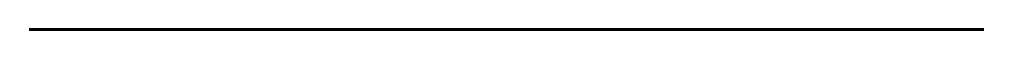
\begin{tikzpicture}
        \draw[very thick] (0,0) -- (\textwidth,0) {};
\end{tikzpicture}\FloatBarrier\parindent 0pt
\bfseries {\huge \sc{Nédélec Space in \texttt{IPPL}}}
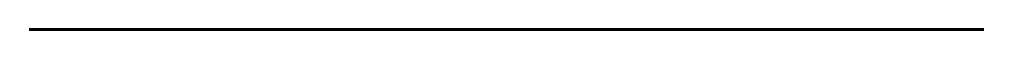
\begin{tikzpicture}
        \draw[very thick] (0,0) -- (\textwidth,0) {};
\end{tikzpicture}\vspace*{-0.5cm}
\begin{figure}[!bh]
        \centering
        \includegraphics[width=0.6\textwidth]{figures/introduction/hero.png}
        %\caption{Vector Field obtained with the Nédélec FEM framework.}
        \label{fig:exampleNedlec}
\end{figure}\vspace*{-1cm}
}

\author{
        \textsc{{{\LARGE Semester Project}}} \\[5pt]
        \small Department of Mathematics \\[5pt] \small ETH Zürich \\
        \vspace{0.5cm} \\
        \normalsize{\sc{written by}} \\[5pt]
        \large{Alexander Pietak} \\ 
        \vspace{0.5cm} \\
        \begin{minipage}{0.5\textwidth}
                \centering
                \normalsize{\sc{supervised by}} \\[5pt]
                \large{Dr.\ A.\ Adelmann (ETH, PSI)}\\
        \end{minipage}
        \begin{minipage}{0.5\textwidth}
                \centering
                \normalsize{\sc{advised by}} \\[5pt]
                \large{S.\ Mayani\ (ETH, PSI)}\\
        \end{minipage}
        \vspace{2cm} \\
        \today
        \vspace*{-20cm}
}
\date{}
% \clearpage
\maketitle
%\thispagestyle{empty}
\end{titlepage}

\setcounter{page}{0}  % set page number -> such that table of contents is first page

%%%%%%%%%%%%%%%%%%%%%%%%%%%%%%%%%%%%%%%%%%%%%%%%%%%%%%%%%%%%%%%%%%%%%%%%%%%%%%%%%%%%%%%%%%%%%%%%%%%%%%%%%%%%%%%%%%%%%%%%%
% ABSTRACT
%%%%%%%%%%%%%%%%%%%%%%%%%%%%%%%%%%%%%%%%%%%%%%%%%%%%%%%%%%%%%%%%%%%%%%%%%%%%%%%%%%%%%%%%%%%%%%%%%%%%%%%%%%%%%%%%%%%%%%%%%

\begin{abstract}

We present a numerical solver for the Vlasov-Poisson equation to simulate plasma dynamics including
Coulomb collisions.
The method makes use of a Langevin type operator to approximate inter-particle collisions via
Rosenbluth potentials.
We employ a Particle-in-Cell approach to efficiently simulate the motion of electrons in a
self-consistent manner.
The governing stochastic differential equation introduces a velocity dependent dynamic friction and
diffusion term accounting for the numerous small angle collisions due to Coulomb repulsion in form of a
stochastic process.

We carry out a thorough study on suitable differential operators for computing the Rosenbluth
potentials as well as the collisional coefficients.
The implementation is subsequently tested on a disorder induced heating process in which particle
collisions play an essential role for the system to attain an equilibrium state.
Additionally, we demonstrate the correctness of the computed collisional terms using analytical test
cases.

\end{abstract}


%%%%%%%%%%%%%%%%%%%%%%%%%%%%%%%%%%%%%%%%%%%%%%%%%%%%%%%%%%%%%%%%%%%%%%%%%%%%%%%%%%%%%%%%%%%%%%%%%%%%%%%%%%%%%%%%%%%%%%%%
% TABLE OF CONTENTS
%%%%%%%%%%%%%%%%%%%%%%%%%%%%%%%%%%%%%%%%%%%%%%%%%%%%%%%%%%%%%%%%%%%%%%%%%%%%%%%%%%%%%%%%%%%%%%%%%%%%%%%%%%%%%%%%%%%%%%%%
\newpage
\pagenumbering{roman}
\tableofcontents


% 27.08.2015, http://tex.stackexchange.com/questions/11579/captions-for-figures-in-listoffigures

% 27.08.2015, https://www.sharelatex.com/learn/Lists_of_tables_and_figures
\listoffigures 
%\listoftables
%\lstlistoflistings
% 06.09.2015, http://tex.stackexchange.com/questions/165903/optional-caption-in-listings-for-listoflistings

%\listofmyoutputs

\newpage
\pagenumbering{arabic}

%%%%%%%%%%%%%%%%%%%%%%%%%%%%%%%%%%%%%%%%%%%%%%%%%%%%%%%%%%%%%%%%%%%%%%%%%%
\chapter{Introduction}
\label{chapter:introduction}

Plasma, often referred to as the fourth state of matter, consists of a gas-like collection of
charged particles (ions and electrons) that exhibit a collective behavior.
Understanding its dynamics under the influence of electric and magnetic fields is of critical
importance for numerous areas in research as well as industry.
A prime example are non-neutral plasmas confined in particle accelerators where particle bunches are exposed to
a range of interesting phenomena which depend on the present plasma state.

In this report, we aim to model a phenomenon arising in ultra-cold plasmas where the transport of
the contained particles is strongly influenced by inter-particle collisions.
Modeling these scattering processes has been an active area of research for many decades
\cite{piwinski1974intra,kubo2001intrabeam}.
The individual scattering events are very weak and often happen over large distances.
Thus, modeling them as binary collisions requires very small timesteps which is not feasible for the
number of particles one usually encounters in dense plasmas.

Instead, researchers have explored methods emanating from plasma kinetic theory which model the scattering
processes via the Fokker-Planck (\gls{fp}) equation \cite{chandrasekhar1943,rosenbluth}.
It can be derived with a Taylor expansion of the statistically averaged effect on the velocity space due to
small-angle deflections. This effect describes advection (via friction) and diffusion in velocity space.
The definition of the friction and diffusion term of the \gls{fp} formalism is not straightforward, thus
researches usually have to state assumptions on the system state in order to approximate them
\cite{manheimer1997langevin,cadjan_ivanov_1999,jonesLangevin_1996}.
In our work we model the collisions via the Langevin formulation of the \gls{fp} equation \cite{cadjan_ivanov_1999}, allowing us to
model them as a stochastic process, providing a velocity dependent
deterministic friction and stochastic diffusion term \cite{stoel}.
This formulation facilitates the use of the Fokker-Planck term as part of the well-established
Particle-in-Cell (\gls{pic}) method \cite{bunemanPIC, dawsonPIC}.

\section{Motivation}

Free Electron Lasers (\gls{fel}) have the ability to generate beams that emit very short coherent light
pulses which exhibit wave lengths down to 0.1\ nm.
This laser is used, among many other applications, to map the atomic structure of proteins with a
high temporal resolution or allows investigating the atomic structure of crystalline matter.
An electron beam is emitted from an electron gun which is subsequently accelerated through an array
of magnets causing a lumping of the beam into bunches.
This process is prone to be negatively impacted by intra-beam scattering of the particles, causing the beam to widen
over time.
As this phenomenon negatively affects the achievable beam brightness, it is important to calibrate an
accelerator to counter this effect as much as possible.

Swiss\gls{fel} is an X-ray \gls{fel} at the Paul Scherrer Institute containing multiple beamlines for producing
many different types of X-ray pulses.
Prat et al. \cite{prat2022energy} have measured in experiments on this machine an energy spread for increased bunch
charges which is a magnitude larger than what their standard simulation codes predicted.
They showed that this blowup is caused mainly by intra-beam scattering and microbunching instabilities.
Being able to model the energy spread correctly is important as it directly influences how much
bunches can be compressed and also defines a lower bound on the achievable wavelength.
An existing method \cite{p3m_ulmer} based on the \gls{p3m} algorithm
(Particle-Particle Particle-Mesh, see Section \ref{section:PIC_method}) has been shown to model
intra-beam collisions adequately, but it does so at a considerable computational cost.
This inhibits simulating bunches over a complete beamline.
The aforementioned method of modeling collisions stochastically via the Langevin formulation promises
better computational complexity, therefore allowing to simulate larger number of particles and simulation domains.
We test the method on an experiment which is governed by disorder induced heating (\gls{dih}) \cite{mitchell2015parallel} and has been
shown to be resolved correctly only if individual particle collisions are considered (via the
\gls{p3m} method \cite{p3m_ulmer}).
This provides us with a challenging test case for the implemented method.

\section{Outline}

We start by introducing the notation used throughout the report, followed by a succinct treatise of the
underlying theory of plasma modeling in the context of kinetic theory, resulting in the Langevin formulation of
the \gls{fp} equation.
Subsequently we discuss the numerical methods used to solve the previously introduced equations and
propose an analytical test case that is used to verify the correctness of our implementation in the following chapter.
We then apply it to the physical test case governed by \gls{dih} and explore what
values the two collisional coefficients attain and how they impact the quantity of normalized emittance.
We conclude this work by highlighting the key findings of our investigation.
Additionally, we propose algorithmic improvements and suggest possible directions for further exploration
of the collisional terms applied in the context of \gls{dih}.

\chapter{Method}
\label{sec:method}
\section{Theory}
\label{subsec:theory}
%\begin{itemize}
%    \item Explain how the IPPL meshes look like.
%    \item How are then the DOFs defined on such elements.
%    \item Write down the local ordering.
%    \item Write down the global ordering.
%    \item Write down conversion formulae.
%    \item Write down the shape function formulas.
%    \item Write down curl of shape function formulas.
%\end{itemize}

\begin{figure}[!ht]
    \centering
    \begin{subfigure}[b]{0.4\textwidth}
        \centering
        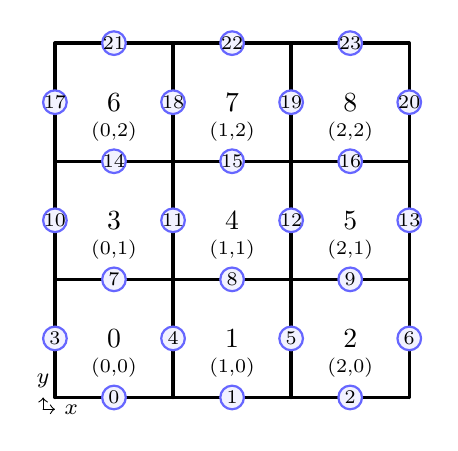
\begin{tikzpicture}[scale=1.5]
    \draw[black, line cap = round, ->] (-0.1,-0.1) -- (0,-0.1) node[color=black, anchor=west] {\footnotesize\(x\)};
    \draw[black, line cap = round, ->] (-0.1,-0.1) -- (-0.1,0) node[color=black, anchor=south] {\footnotesize\(y\)};
    
    \draw[black, very thick, line cap = round] (0,3) -- (3,3);
    \draw[black, very thick, line cap = round] (3,0) -- (3,3);

    \foreach \x in {0,...,2}
        \foreach \y in {0,...,2} 
            {\draw[black, very thick, line cap = round] (\x,\y) -- (\x,\y+1);
             \draw[black, very thick, line cap = round] (\x,\y) -- (\x+1,\y);
             \filldraw[color=blue!60, fill=blue!5, thick](\x + 0.5,\y) circle (0.1) node[color=black] {\scriptsize$\the\numexpr\x+\y*7\relax$};
             \filldraw[color=blue!60, fill=blue!5, thick](\x,\y + 0.5) circle (0.1) node[color=black] {\scriptsize$\the\numexpr\x+\y*7+3\relax$};
             \ifthenelse{2 = \x}{\filldraw[color=blue!60, fill=blue!5, thick](\x+1,\y + 0.5) circle (0.1) node[color=black] {\scriptsize$\the\numexpr\x+\y*7+4\relax$}}{};
             \ifthenelse{2 = \y}{\filldraw[color=blue!60, fill=blue!5, thick](\x+0.5,\y + 1) circle (0.1) node[color=black] {\scriptsize$\the\numexpr\x+(\y+1)*7\relax$}}{};
             \node[] at (\x+0.5,\y+0.5) (a) {$\the\numexpr\y*3 + \x\relax$};
             \node[] at (\x+0.5,\y+0.25) {\scriptsize(\x,\y)};}


\end{tikzpicture}
        \caption{Global DOF numbering scheme, element numbering, and multidimensional index in 2D, for a \(4 \times 4\) mesh.}
    \end{subfigure}
    \hspace{0.08\textwidth}
    \begin{subfigure}[b]{0.4\textwidth}
        \centering
        \tdplotsetmaincoords{70}{15}
\begin{tikzpicture}[scale=1.8,tdplot_main_coords]
    \draw[black, line cap = round, ->] (-0.2,-0.2,-0.2) -- (0,-0.2,-0.2) node[color=black, anchor=west] {\footnotesize\(x\)};
    \draw[black, line cap = round, ->] (-0.2,-0.2,-0.2) -- (-0.2,0,-0.2) node[color=black, anchor=south west] {\footnotesize\(y\)};
    \draw[black, line cap = round, ->] (-0.2,-0.2,-0.2) -- (-0.2,-0.2,0) node[color=black, anchor=south] {\footnotesize\(z\)};
    

    
    
    \foreach \y in {1,0} {
        \foreach \z in {0,...,1} {
            \foreach \x in {0,...,1} {
                %\node[] at (\x+0.5,\y+0.5,\z+0.5) {$\the\numexpr\z*4 + \y*2 + \x\relax$};
                %\node[] at (\x+0.5,\y+0.5,\z+0.25) { \scriptsize(\x,\y,\z)};

                \ifthenelse{1 = \y}{
                    \draw[black, very thick, line cap = round] (\x,\y+1,\z) -- (\x+1,\y+1,\z);
                    \draw[black, very thick, line cap = round] (\x,\y+1,\z) -- (\x,\y+1,\z+1);

                    \filldraw[color=blue!60, fill=blue!5, thick](\x+0.5,\y+1,\z) circle (0.1cm) node[color=black] {\scriptsize$\the\numexpr\x+\y*5+\z*21+5\relax$};
                    \filldraw[color=blue!60, fill=blue!5, thick](\x,\y+1,\z+0.5) circle (0.1cm) node[color=black] {\scriptsize$\the\numexpr\z*21+12+\y*3+\x+3\relax$};
                }{};

                \draw[black, very thick, line cap = round] (\x,\y,\z) -- (\x,\y+1,\z);
                \draw[black, very thick, line cap = round] (\x,\y,\z) -- (\x+1,\y,\z);
                \draw[black, very thick, line cap = round] (\x,\y,\z) -- (\x,\y,\z+1);
                \filldraw[color=blue!60, fill=blue!5, thick](\x + 0.5,\y,\z) circle (0.1cm) node[color=black] {\scriptsize$\the\numexpr\x+\y*5+\z*21\relax$};
                \filldraw[color=blue!60, fill=blue!5, thick](\x,\y + 0.5,\z) circle (0.1cm) node[color=black] {\scriptsize$\the\numexpr\x+\y*5+\z*21+2\relax$};
                \filldraw[color=blue!60, fill=blue!5, thick](\x,\y,\z + 0.5) circle (0.1cm) node[color=black] {\scriptsize$\the\numexpr\z*21+12+\y*3+\x\relax$};
                

                \ifthenelse{1 = \z}{
                    \draw[black, very thick, line cap = round] (\x,\y,\z+1) -- (\x,\y+1,\z+1);
                    \draw[black, very thick, line cap = round] (\x,\y,\z+1) -- (\x+1,\y,\z+1);

                    \filldraw[color=blue!60, fill=blue!5, thick](\x+0.5,\y,\z+1) circle (0.1cm) node[color=black] {\scriptsize$\the\numexpr\x+\y*5+\z*21+21\relax$};
                    \filldraw[color=blue!60, fill=blue!5, thick](\x,\y+0.5,\z+1) circle (0.1cm) node[color=black] {\scriptsize$\the\numexpr\x+\y*5+\z*21+23\relax$};
                }{};



                \ifthenelse{1 = \x}{
                    \draw[black, very thick, line cap = round] (\x+1,\y,\z) -- (\x+1,\y+1,\z);
                    \draw[black, very thick, line cap = round] (\x+1,\y,\z) -- (\x+1,\y,\z+1);

                    \filldraw[color=blue!60, fill=blue!5, thick](\x+1,\y+0.5,\z) circle (0.1cm) node[color=black] {\scriptsize$\the\numexpr\x+\y*5+\z*21+3\relax$};
                    \filldraw[color=blue!60, fill=blue!5, thick](\x+1,\y,\z+0.5) circle (0.1cm) node[color=black] {\scriptsize$\the\numexpr\z*21+12+\y*3+\x+1\relax$};
                }{};

                \ifthenelse{1 = \x \AND 1 = \y}{
                    \draw[black, very thick, line cap = round] (\x+1,\y+1,\z) -- (\x+1,\y+1,\z+1);
                    \filldraw[color=blue!60, fill=blue!5, thick](\x+1,\y+1,\z+0.5) circle (0.1cm) node[color=black] {\scriptsize$\the\numexpr\z*21+12+\y*3+\x+4\relax$};
                }{}
                \ifthenelse{1 = \x \AND 1 = \z}{
                    \draw[black, very thick, line cap = round] (\x+1,\y,\z+1) -- (\x+1,\y+1,\z+1);
                    \filldraw[color=blue!60, fill=blue!5, thick](\x+1,\y+0.5,\z+1) circle (0.1cm) node[color=black] {\scriptsize$\the\numexpr\x+\y*5+\z*21+24\relax$};
                }{}
                \ifthenelse{1 = \y \AND 1 = \z}{
                    \draw[black, very thick, line cap = round] (\x,\y+1,\z+1) -- (\x+1,\y+1,\z+1);
                    \filldraw[color=blue!60, fill=blue!5, thick](\x+0.5,\y+1,\z+1) circle (0.1cm) node[color=black] {\scriptsize$\the\numexpr\x+\y*5+\z*21+26\relax$};
                }{}
            }
        }
    }
            


\end{tikzpicture}
        \caption{Global DOF numbering scheme for 3D, given for a \(3 \times 3 \times 3\) mesh.}
    \end{subfigure}
    \caption{The global DOF numbering scheme (blue circles) for the Nédélec space in both 2D and 3D. For 2D also the element numbering (black number), and its multidimensional index (black pair) is given, for 3D this was omitted for visual clarity.}
    \label{fig:glob_numbering}
\end{figure}

\begin{figure}[!ht]
    \centering
    \begin{subfigure}[b]{0.4\textwidth}
        \centering
        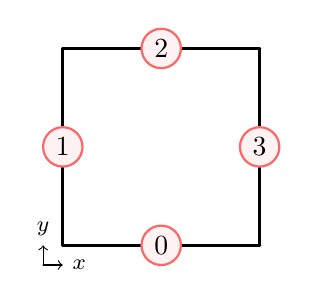
\begin{tikzpicture}[scale=2.5]
    \draw[black, line cap = round, ->] (-0.1,-0.1) -- (0,-0.1) node[color=black, anchor=west] {\footnotesize\(x\)};
    \draw[black, line cap = round, ->] (-0.1,-0.1) -- (-0.1,0) node[color=black, anchor=south] {\footnotesize\(y\)};

    \draw[black, very thick, line cap = round] (0,0) -- (1,0);
    \draw[black, very thick, line cap = round] (0,0) -- (0,1);
    \draw[black, very thick, line cap = round] (1,0) -- (1,1);
    \draw[black, very thick, line cap = round] (0,1) -- (1,1);

    \filldraw[color=red!60, fill=red!5, thick](0.5,0) circle (0.1) node[color=black] {0};
    \filldraw[color=red!60, fill=red!5, thick](0,0.5) circle (0.1) node[color=black] {1};
    \filldraw[color=red!60, fill=red!5, thick](0.5,1) circle (0.1) node[color=black] {2};
    \filldraw[color=red!60, fill=red!5, thick](1,0.5) circle (0.1) node[color=black] {3};
\end{tikzpicture}
        \caption{The reference element for the 2D case, with the local DOF numbering.}
    \end{subfigure}
    \hspace{0.08\textwidth}
    \begin{subfigure}[b]{0.4\textwidth}
        \centering
        \tdplotsetmaincoords{70}{15}
\begin{tikzpicture}[scale=2.5,tdplot_main_coords]

    \draw[black, line cap = round, ->] (-0.1,-0.1,-0.1) -- (0,-0.1,-0.1) node[color=black, anchor=west] {\footnotesize\(x\)};
    \draw[black, line cap = round, ->] (-0.1,-0.1,-0.1) -- (-0.1,0,-0.1) node[color=black, anchor=south west] {\footnotesize\(y\)};
    \draw[black, line cap = round, ->] (-0.1,-0.1,-0.1) -- (-0.1,-0.1,0) node[color=black, anchor=south] {\footnotesize\(z\)};



    \draw[black, very thick, line cap = round] (0,0,0) -- (1,0,0);
    \draw[black, very thick, line cap = round] (0,0,0) -- (0,1,0);
    \draw[black, very thick, line cap = round] (1,0,0) -- (1,1,0);
    \draw[black, very thick, line cap = round] (0,1,0) -- (1,1,0);
    \draw[black, very thick, line cap = round] (0,0,1) -- (1,0,1);
    \draw[black, very thick, line cap = round] (0,0,1) -- (0,1,1);
    \draw[black, very thick, line cap = round] (1,0,1) -- (1,1,1);
    \draw[black, very thick, line cap = round] (0,1,1) -- (1,1,1);
    
    \draw[black, very thick, line cap = round] (0,0,0) -- (0,0,1);
    \draw[black, very thick, line cap = round] (0,1,0) -- (0,1,1);
    \draw[black, very thick, line cap = round] (1,0,0) -- (1,0,1);
    \draw[black, very thick, line cap = round] (1,1,0) -- (1,1,1);


    \filldraw[color=red!60, fill=red!5, thick](0.5,0,0) circle (0.1cm) node[color=black] {0};
    \filldraw[color=red!60, fill=red!5, thick](0,0.5,0) circle (0.1cm) node[color=black] {1};
    \filldraw[color=red!60, fill=red!5, thick](0.5,1,0) circle (0.1cm) node[color=black] {2};
    \filldraw[color=red!60, fill=red!5, thick](1,0.5,0) circle (0.1cm) node[color=black] {3};
    \filldraw[color=red!60, fill=red!5, thick](0,0,0.5) circle (0.1cm) node[color=black] {4};
    \filldraw[color=red!60, fill=red!5, thick](1,0,0.5) circle (0.1cm) node[color=black] {5};
    \filldraw[color=red!60, fill=red!5, thick](1,1,0.5) circle (0.1cm) node[color=black] {6};
    \filldraw[color=red!60, fill=red!5, thick](0,1,0.5) circle (0.1cm) node[color=black] {7};
    \filldraw[color=red!60, fill=red!5, thick](0.5,0,1) circle (0.1cm) node[color=black] {8};
    \filldraw[color=red!60, fill=red!5, thick](0,0.5,1) circle (0.1cm) node[color=black] {9};
    \filldraw[color=red!60, fill=red!5, thick](0.5,1,1) circle (0.1cm) node[color=black] {10};
    \filldraw[color=red!60, fill=red!5, thick](1,0.5,1) circle (0.1cm) node[color=black] {11};
\end{tikzpicture}
        \caption{The reference element for the 3D case, with the local DOF numbering.}
    \end{subfigure}
    \caption{The reference elements for the Nédélec space in both 2D and 3D with the DOF numbering scheme.}
    \label{fig:ref_elements}
\end{figure}

Currently \texttt{IPPL} only supports structured, rectilinear grid meshes. Therefore our FEM reference elements are the unit square in 2D and the unit cube in 3D, for which our Nédélec Degrees of Freedom (DOFs) reside on the edges. In order to be able to interact with them we assign each DOF a number, this numbering happens by sorting, low to high, the DOF positions according to first their \(z\)-coordinate (only in 3D), because there are multiple DOFs with same \(z\)-coordinate we have not created a unique ordering, but a block ordering, where we have multiple blocks of DOFs with same \(z\)-coordinate and these blocks are sorted correctly. Then in order to further sort we now take each of these blocks and sort them according to their \(y\)-coordinate (in 2D we would simply start here and order all DOFs according to their \(y\)-coordinate), but this again will create a block sorting for which we then sort each block according to their \(x\)-coordinate. After we have sorted the final blocks according to \(x\) we now should have created an unique ordering of the DOFs. An example can be seen in Figure \ref{fig:glob_numbering}. The elements are numbered in the same manner, but additionally also have a multidimensional index, which is a coordinate vector \(\vec p\), that tells the position of an element relative to the mesh itself, so it gives you the offset in elements of an element relative to the element with smallest position, this can also be seen in Figure \ref{fig:glob_numbering}. During the FEM calculations we are going to work with a reference element, which in our case is either the unit square or the unit cube. On it we are also going to have to number the local DOFs, this is given in Figure \ref{fig:ref_elements}. This notion of local numbering does not only apply to the reference element, but also for the elements inside of the mesh, where the local DOFs are simply the ones which lie on this element.\medskip

During the FEM calculations we are often required to retrieve the global shape functions associated with an element given by its multidimensional index, in other words: figuring out what the global indices of the local shape functions of an element are. The global DOF indices for an element with multidimensional index \(\vec{p}\) living in a mesh with number of vertices per axis given by \(n_x\), \(n_y\), and \(n_z\) are given in Equation (\ref{eq:el2glob2d}) for the 2D case and in Equation (\ref{eq:el2glob3d}) for 3D, where they are ordered according to the local shape functions.
\begin{align}
    \text{DOFs} =
    \begin{bNiceMatrix}
        a \\ b \\ c \\ d
    \end{bNiceMatrix} = 
    \begin{bNiceMatrix}[l]
        \vec{v} \cdot \vec{p} \\
        a + n_x - 1 \\
        b + n_x \\
        b + 1
    \end{bNiceMatrix}, \text{ with } \vec{v} =
    \begin{bNiceMatrix}
        1 \\ 2n_x -1
    \end{bNiceMatrix} \label{eq:el2glob2d}
\end{align}

\begin{align}
    \text{DOFs} =
    \begin{bNiceMatrix}
        a \\ b \\ c \\ d \\ e \\ f \\ g \\ h \\ i \\ j \\ k \\ l
    \end{bNiceMatrix} = 
    \begin{bNiceMatrix}[l]
        \vec{v} \cdot \vec{p} \\
        a + n_x - 1\\
        b + n_x \\
        b + 1 \\
        \vec{v}_z \vec{p}_z + 2 n_x n_y - n_x - n_y + \vec{p}_y n_x + \vec{p}_x \\
        e + 1 \\
        e + n_x \\
        e + n_x + 1 \\
        a + 3n_x n_y - n_x -n_y \\
        i + n_x -1 \\
        j + n_x \\
        j+1
    \end{bNiceMatrix}, \text{ with } \vec{v} =
    \begin{bNiceMatrix}
        1 \\ 2n_x -1 \\ 3n_x n_y - n_x - n_y
    \end{bNiceMatrix}\label{eq:el2glob3d}
\end{align}\medskip

The last thing left to do is to the state the formulae for the basis functions. Here we follow standard FEM methodology and do not evaluate the basis functions on the mesh, but define a reference element on which we evaluate them and then use a transformation in order to transform them to the actual element in the mesh. We define with \(\vec \beta_i\) the \(i\)-th local shape function, \(i \in \{0,1,2,3\}\) for 2D and \(i \in \{0,1,2,...,11\}\) for 3D, of an element in the mesh, and with \(\hat{\vec{\beta}}_i\) the corresponding shape function in the reference element. The formulae for the \(\hat{\vec{\beta}}_i\) are readily available, such as in \cite{maxwellBook}, and they are given in Collection \ref{tab:shape_funcs}. So we want to evaluate the function \(f(\cdot)\), which depends on the shape function \(\vec\beta_i\) transformed by an arbitrary operator \(\mathcal{L}\), i.e., \(f(\mathcal L \circ \vec \beta_i)\), using the reference element shape functions, such that we get:
\begin{align}
    f(\mathcal L \circ \vec \beta_i) = f(\mathcal{G} \circ (\mathcal L \circ \hat{\vec{\beta}}_i))\text{,}
\end{align}
where \(\mathcal{G}\) is the operator that we are looking for. In the case of curl-conforming Nédélec space \(\mathcal{L}\) will in most cases either be identity or the curl operator, for them we have that the \(\mathcal{G}\) will look as follows:
\begin{align}
    f(\vec \beta_i) &= f(\hat{\vec{\beta}}_i) \text{ and } \\
    f(\nabla \times \vec \beta_i) &= f(J^{-T} (\nabla \times \hat{\vec{\beta}}_i))\text{,}
\end{align}
so in the case of identity \(\mathcal{G}\) is identity and for the curl it is \(J^{-T}\), which is the inverse transpose Jacobian of the affine transformation between the reference element and the actual element.

\begin{table}[!ht]
    \centering
    2D
    \begin{multicols}{4}
    \begin{itemize}
        \item[] \(\hat{\vec{\beta}}_0 = \begin{bmatrix}1 - y \\ 0\end{bmatrix}\),
        \item[] \(\hat{\vec{\beta}}_1 = \begin{bmatrix}0 \\ 1 - x\end{bmatrix}\),
        \item[] \(\hat{\vec{\beta}}_2 = \begin{bmatrix}y \\ 0\end{bmatrix}\),
        \item[] \(\hat{\vec{\beta}}_3 = \begin{bmatrix}0 \\ x\end{bmatrix}\).
    \end{itemize}
    \end{multicols}
    
    \vspace{0.5cm}
    
    3D
    \begin{multicols}{3}
    \begin{itemize}
        \item[] $\hat{\vec{\beta}}_0$ = $\begin{bmatrix}yz - y - z + 1 \\ 0 \\ 0\end{bmatrix}$, \\
        \item[] $\hat{\vec{\beta}}_1$ = $\begin{bmatrix}0 \\ xz - x - z + 1 \\ 0\end{bmatrix}$, \\
        \item[] $\hat{\vec{\beta}}_2$ = $\begin{bmatrix}y(1-z) \\ 0 \\ 0\end{bmatrix}$, \\
        \item[] $\hat{\vec{\beta}}_3$ = $\begin{bmatrix}0 \\ x(1-z) \\ 0\end{bmatrix}$, \\
        \item[] $\hat{\vec{\beta}}_4$ = $\begin{bmatrix}0 \\ 0 \\ xy - x - y +1\end{bmatrix}$, \\
        \item[] $\hat{\vec{\beta}}_5$ = $\begin{bmatrix}0 \\ 0 \\ x(1-y)\end{bmatrix}$, \\
        \item[] $\hat{\vec{\beta}}_6$ = $\begin{bmatrix}0 \\ 0 \\ xy\end{bmatrix}$, \\
        \item[] $\hat{\vec{\beta}}_7$ = $\begin{bmatrix}0 \\ 0 \\ y(1-x)\end{bmatrix}$, \\
        \item[] $\hat{\vec{\beta}}_8$ = $\begin{bmatrix}z(1-y) \\ 0 \\ 0\end{bmatrix}$, \\
        \item[] $\hat{\vec{\beta}}_9$ = $\begin{bmatrix}0 \\ z(1-x) \\ 0\end{bmatrix}$, \\
        \item[] $\hat{\vec{\beta}}_{10}$ = $\begin{bmatrix}yz \\ 0 \\ 0\end{bmatrix}$, \\
        \item[] $\hat{\vec{\beta}}_{11}$ = $\begin{bmatrix}0 \\ xz \\ 0\end{bmatrix}$. \\
    \end{itemize}
    \end{multicols}
    \renewcommand{\tablename}{Collection}
    \caption{Formulae for the local shape functions on the reference element of the Nédélec space in both 2D and 3D.}
    \renewcommand{\tablename}{Table}
    \label{tab:shape_funcs}
\end{table}


\section{Pipeline}
%\begin{itemize}
%    \item General pipeline (solver, Nédélec space,...).
%    \item Explain what type of problem we can solve \(F(u) = g \text{ in } \Omega\), with \(u\times n = 0 \text{ on } \partial \Omega \).
%    \item Have diagram explaining it.
%    \item PIC provides rhs \(g\), get passed to a solver (which solves one specific type of problem), solver interacts with Nédélec space in order to obtain rhs and Ax, solver calls CG to solve Ax=b, solver provides coefficients.
%    \item Talk about matrix-free-ness.
%    \item Therefore need solver and Nédélec space class.
%    \item Additionally problem of how store x and b \(\implies\) need FEMVector.
%    \item These are all the building blocks required.
%\end{itemize}
\begin{figure}[!h]
    \centering
    \input{figures/method/pipeline.tex}
    \caption{General pipeline diagram, for the solving of a problem using the Nédélec space.}
    \label{fig:gen_diag}
\end{figure}
The general pipeline we are using is shown in Figure \ref{fig:gen_diag}. We define a solver, to solve a problem for $\vec{u}(\vec{x})$ of the form:
\begin{align}
    &F(\vec{u}(\vec{x})) = \vec{g}(\vec{x}) \text{ in } \Omega\text{,} \\
    &\vec{u}(\vec{x}) \times \vec{n} = 0 \text{ on } \partial \Omega \text{,}
\end{align}
where $F(\cdot)$ defines some functional which determines the type of problem we are solving, $\vec{g}(\cdot)$ is the right hand side (RHS) function, and $\vec{n}$ is the normal vector of the domain $\Omega$.\medskip

The first step of the pipeline regards the right hand side function $\vec{g}$, which will be provided to us, in some form, by the PIC code; We will later go into more detail on the exact way in which we represent this RHS. The next step in the pipeline consists of assembling the Galerkin system $A\vec{\mu} = \vec{b}$, where $A$ is defined by $F(\cdot)$, $\vec{b}$ by \(\vec g\), and \(\vec\mu\) is the solution vector. During the assembly is where the finite element space comes into play, in our case this is the \texttt{NedelecSpace} class, as it knows about how the Galerkin discretization looks like and therefore how the matrix \(A\) and the vector \(\vec b\) need to be constructed. Note that in our case we are doing this matrix-free, so instead of fully expressing the entries of the matrix $A$ we construct a functional which returns the result of the multiplication $A\vec{v}$ for some arbitrary vector $\vec{v}$, as such a multiplication is the only information needed to solve such a system using the Conjugate Gradient (CG) method. When the information about the linear system is created we pass it to the CG solver, which will then solve it for us and returns the solution vector $\vec{\mu}$. Note that the solution vector $\vec{\mu}$ only stores the basis function coefficients of the Nédélec space and in order to retrieve the solution $\vec{u}(\vec{x})$ we have to reconstruct it, something which is done by the Nédélec space. After all this is done we can pass the solution back to PIC and we are done with the FEM-based solve.\medskip

One question we have to answer is how we store the vectors $\vec{b}$ and $\vec{\mu}$. Both of them are 1D vector which store values at the DOF positions and which need to provide functionality for halo exchanges and domain boundaries. Until now \texttt{IPPL} only supported the first order Lagrangian space, where the DOF positions coincide with the vertex positions and therefore an \texttt{ippl::Field} could be used, which is a data structure containing values at the mesh grid-points, i.e., vertex positions. However, for the Nédélec space the DOFs are edge centered and therefore cannot be stored inside of an \texttt{ippl::Field}. To this end we implemented a new class called \texttt{FEMVector}, which represents a 1D vector and provides functionality for halo exchanges (currently no boundary operations are implemented).\medskip

With this general overview provided, we will now discuss in more detail the different parts of the pipeline.

\section{FEMVector}
%\begin{itemize}
%    \item Explain basic principle behind FEMVector.
%    \item Go into implementation details.
%    \item Explain how halo exchange is implement.
%    \item Talk about fact, that FEMVector is general object, but each one has to be specifically tailored to a space, due to the halo exchange, boundary, and mapping from index to DOF.
%\end{itemize}
\begin{figure}[!ht]
    \centering
    \begin{tikzpicture}[scale=1.5]
    \tikzumlset{fill class=red!5, draw=red!60, class width=20ex}
    \umlclass{ippl::FEMVector}{
        - data: Kokkos::View
    }{
        %+ FEMVector()\\
        + fillHalo()\\
        + accumulateHalo()\\
        + setHalo()\\
        %+ operator=()\\
        %+ operator[]()\\
        %+ operator()()\\
        %+ getView()\\
        %+ size() \\
        + deepCopy()\\
        + skeletonCopy()\\
        %- pack()\\
        %- unpack()\\
        ...
    }

    \umlsimpleclass[y=3,x=-2]{ippl::detail::Expression}

    \umlclass[y=3,x=4]{ippl::FEMVector::BoundaryInfo}{
        + neighbors\\
        + sendIdxs \\
        + recvIdxs
    }{
        %+ BoundaryInfo()\\
    }

    \umlinherit{ippl::FEMVector}{ippl::detail::Expression}
    \umlaggreg [mult1=-boundaryInfo]{ippl::FEMVector}{ippl::FEMVector::BoundaryInfo}
\end{tikzpicture}

    \caption{UML Class diagram for the \texttt{FEMVector}.}
    \label{fig:uml_femvector}
\end{figure}
In its very core the \texttt{FEMVector}, Figure \ref{fig:uml_femvector}, is a wrapper around a 1D \texttt{Kokkos::View} which stores data of a templated type. So the \texttt{FEMVector} has a member called \texttt{data} which is a 1D \texttt{Kokkos::View} and then some methods to interact with it, like retrieving its size, an entry, or even itself. While this is neither revolutionary, nor particularly useful, its actual usefulness comes from its ability to perform halo operations (used during parallelization with MPI). Additionally it also allows for the future implementation of new features, like the handling of domain boundaries.\medskip

In order to allow for the halo exchange the \texttt{FEMVector} exposes a set of functions to manipulate the halo, namely \texttt{fillHalo()}, \texttt{accumulateHalo()}, and \texttt{setHalo()}, where the first two are equivalent to their \texttt{ippl::Field} counter parts and the third one is used to set the value of the halo to what is passed as an argument. The way in which the halo is internally handled is by having three lists, the first one, called \texttt{neighbors}, simply stores the MPI ranks of all the other ranks from which information needs to be send or received. The other two lists, called \texttt{sendIdxs} and \texttt{recvIdxs}, are lists of lists which store for each rank in \texttt{neighbors} a list of indices of the underlying \texttt{Kokkos::View}, which are part of their halo and we therefore have to send (\texttt{sendIdxs}), or which are part of our halo and we therefore have to receive values into (\texttt{recvIdxs}). All these lists are passed to the \texttt{FEMVector} at construction time. As we are simply working with indices we are able to create an exchange mechanism that is completely independent of the underlying geometry of the problem and by already passing the lists in the constructor we can also have that the \texttt{FEMVector} is completely unaware of the geometry it is used upon, which adds flexibility.\medskip

These three lists are implemented using a \texttt{std::vector<size\_t>} for \texttt{neighbors} and a \texttt{std::vector<Kokkos::View<size\_t*>>} for both \texttt{sendIdxs} and \texttt{recvIdxs}. They are not directly stored inside of the \texttt{FEMVector} class, but inside of a helper struct, called \texttt{BoundaryInfo}, to which the \texttt{FEMVector} owns a pointer. The reason for having this separation between the \texttt{FEMVector} with its boundary exchange logic and the \texttt{BoundaryInfo} with the data needed to perform the exchange is to have a smaller footprint of the \texttt{FEMVector}, allowing for cheaper copying to device, and for the easy creation of \texttt{FEMVector}s which do not have any halo information; of course this means that when the entire \texttt{FEMVector} is copied to device any information about the boundary is lost. On the other hand we still have that the exchange of data needs to happen via the device, as the entries of the \texttt{FEMVector} are stored there, this is the reason why the \texttt{sendIdxs} and \texttt{recvIdxs} store \texttt{Kokkos::Views}, which then are passed (in the form of \texttt{Kokkos::View}s) by the CPU to the GPU during the exchange. The actual exchange logic then becomes rather trivial, and consists of looping over the entries in \texttt{neighbors} and for each of them copy data, on the device, according to either \texttt{sendIdxs} or \texttt{recvIdxs} to a buffer which then is sent over the network. For receiving we again loop over the \texttt{neighbors}, receive into the buffer and then copy into the \texttt{FEMVector} data according to either \texttt{sendIdxs} or \texttt{recvIdxs}. The logic used to handle the buffer is equivalent to the one utilized by the \texttt{ippl::HaloCells} class, which can be found in \cite{matthias_frey_2024_10878166}, and will therefore not be discussed in detail.\medskip

The last important thing that the \texttt{FEMVector} provides are methods for copying, namely a function called \texttt{deepCopy()} and one called \texttt{skeletonCopy()}. The function \texttt{deepCopy()} creates a new \texttt{FEMVector} which is identical to the current one and stores the same values. The function \texttt{skeletonCopy()} on the other hand will not copy over the values, it creates a new \texttt{FEMVector} of same size and boundary info, but it takes a template parameter which sets the value-type of the entries of the new object, allowing for the creation of a \texttt{FEMVector} with same structure, but which stores different types of values. This becomes especially useful when dealing with both \texttt{FEMVectors} that need to store vectors and \texttt{FEMVectors} that need to store scalars.\medskip

From all this we can see that the \texttt{FEMVector} is a general object, which is independent from any sort of mesh, DOFs, MPI layout, or even FEM itself. Meaning, that it can be utilized in a lot of different situations, from higher order Lagrange, to new finite element spaces, or something completely independent of FEM like general mesh data that needs to support communication, but this flexibility also means that when we use a \texttt{FEMVector} we need to create a supporting structure around it, that relates the \texttt{FEMVector} to its use case. This structure has to mainly provide two things, the first one is functionality to map between the entries of the \texttt{FEMVector} and the DOFs (or arbitrary points) inside of the mesh, and the second one is functionality to create \texttt{FEMVector}s, this includes figuring out the correct size and setting-up all the halo exchange information, given some representation of the MPI domain decomposition. So while the \texttt{FEMVector} is a general object we still need to custom tailor it to the use-case that we have, which in our case is all part of the Nédélec space.

\section{Nédélec Space}
%\begin{itemize}
%    \item Class storing all the information about the Nédélec space. Basis function information (formula, mapping from global to local index, curls,...), provides methods for the creation of FEMVectors, provides method for the evaluation of the rhs (currently given Functional for \(g\)), provides method for the Ax evaluation given some description of \(F(u)\) by the solver.
%    \item Provides some additional helper things like error metrics.
%\end{itemize}
\begin{figure}[!ht]
    \centering
    \begin{tikzpicture}[scale=1.5]
    \tikzumlset{fill class=red!5, draw=red!60, class width=20ex}
    \umlclass{ippl::NedelecSpace}{
        ...
    }{
        + getGlobalDOFIndices()\\
        + getFEMVectorDOFIndices()\\
        + evaluateAx()\\
        + evaluateLoadVector()\\
        + createFEMVector()\\
        + computeError()\\
        + reconstructToPoints()\\
        ...
    }

    \umlsimpleclass[y=3,x=-2]{ippl::FiniteElementSpace}


    \umlinherit{ippl::FEMVector}{ippl::FiniteElementSpace}

\end{tikzpicture}
    \caption{UML Class diagram for the Nédélec Space.}
    \label{fig:uml_nedelec_space}
\end{figure}
The \texttt{NedelecSpace} class (UML diagram in Figure \ref{fig:uml_nedelec_space}) stores all the information regarding the Nédélec space. This means all the information about the basis functions, from the mapping between global and local index to their formula and their curl. It provides methods for the evaluation of the RHS given a representation of \(g(\vec{x})\) and the evaluation of the multiplication \(A\vec{v}\), between the Galerkin matrix and an arbitrary vector. It also creates the supporting structure around the \texttt{FEMVector}, namely the mapping between the DOF indices and the entries of the \texttt{FEMVector}, as well as routines for the creation of \texttt{FEMVector}s. Lastly it provides functionality for the calculation of the L2 error, given an analytical form, and the reconstruction of the solution given the Nédélec basis coefficients. All these points are discussed in more detail in the next few sections.


\subsection{Basis Functions}
%\begin{itemize}
%    \item More information about what we store about the basis functions.
%    \item Mostly references to theory part.
%\end{itemize}
As already mentioned we store information regarding the mapping from local to global DOFs, this equates to implementing the formulae defined in Equations (\ref{eq:el2glob2d}) and (\ref{eq:el2glob3d}). Similarly we also have methods to retrieve the shape function values at arbitrary points inside of the reference element, which is laid out by Collection (\ref{tab:shape_funcs}). Next to simply retrieving the shape function values we also need the curl of it, defined by $\nabla \times \vec{\beta}_i$ with $\vec{\beta}_i$ the $i$-th basis function, as this is one of the most common operators needed in curl-conforming Nédélec FEM. In the future different operators can be implemented depending on what the problem to solve requires, as different PDEs require different operators.


\subsection{FEMVector}
\label{subsubsec:femvector}
%\begin{itemize}
%    \item Talk about order in which we store the DOFs in the FEMVector, also with regard to multirank.
%    \item Talk about how the halo boundaries look like.
%    \item Talk about what we need to exchange.
%    \item Talk about fact, that we do not exchange some of the diagonals, but that it still works.
%\end{itemize}
\begin{figure}
    \centering
    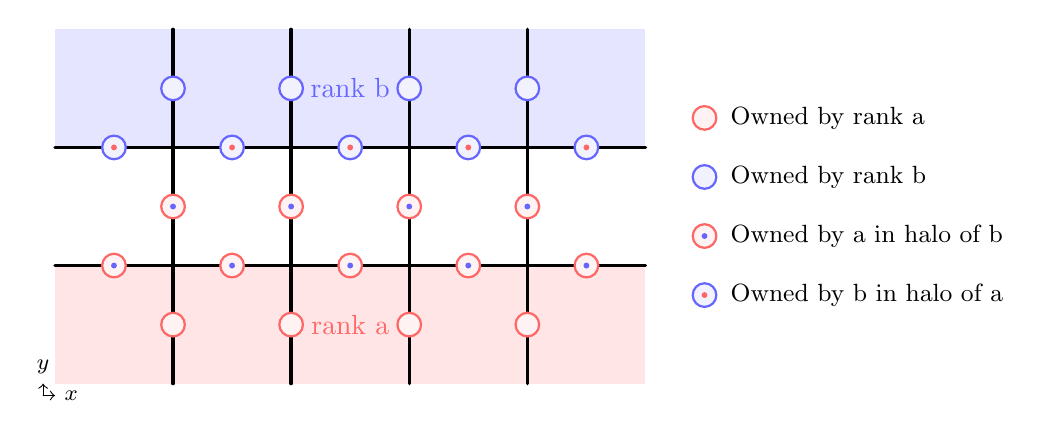
\begin{tikzpicture}[scale=1.5]
    \draw[black, line cap = round, ->] (-0.1,-0.1) -- (0,-0.1) node[color=black, anchor=west] {\footnotesize\(x\)};
    \draw[black, line cap = round, ->] (-0.1,-0.1) -- (-0.1,0) node[color=black, anchor=south] {\footnotesize\(y\)};
    
    %\fill [shading = axis, top color=red!50, bottom color=white, color=red!90] (0,0) rectangle (5,1) node[pos=0.5] {rank a};
    %\fill [shading = axis, bottom color=blue!50, top color=white, color=blue!90] (0,2) rectangle (5,3) node[pos=0.5] {rank b};
    \fill[fill=red!10] (0,0) rectangle (5,1) node[pos=0.5, color=red!60] {rank a};
    \fill[fill=blue!10] (0,2) rectangle (5,3) node[pos=0.5, color=blue!60] {rank b};

    % Horizontal lines
    %\draw[black, very thick, line cap = round] (0,0) -- (5,0);
    \draw[black, very thick, line cap = round] (0,1) -- (5,1);
    \draw[black, very thick, line cap = round] (0,2) -- (5,2);
    %\draw[black, very thick, line cap = round] (0,3) -- (5,3);

    % vertical lines
    %\draw[black, very thick, line cap = round] (0,0) -- (0,3);
    \draw[black, very thick, line cap = round] (1,0) -- (1,3);
    \draw[black, very thick, line cap = round] (2,0) -- (2,3);
    \draw[black, very thick, line cap = round] (3,0) -- (3,3);
    \draw[black, very thick, line cap = round] (4,0) -- (4,3);


    % rank a DOFs
    \filldraw[color=red!60, fill=red!5, thick](1,0.5) circle (0.1) node[color=black] {};
    \filldraw[color=red!60, fill=red!5, thick](2,0.5) circle (0.1) node[color=black] {};
    \filldraw[color=red!60, fill=red!5, thick](3,0.5) circle (0.1) node[color=black] {};
    \filldraw[color=red!60, fill=red!5, thick](4,0.5) circle (0.1) node[color=black] {};
    \filldraw[color=red!60, fill=red!5, thick](0.5,1) circle (0.1);
    \fill[fill=blue!60] (0.5,1) circle (0.025);
    \filldraw[color=red!60, fill=red!5, thick](1.5,1) circle (0.1) node[color=black] {};
    \fill[fill=blue!60] (1.5,1) circle (0.025);
    \filldraw[color=red!60, fill=red!5, thick](2.5,1) circle (0.1) node[color=black] {};
    \fill[fill=blue!60] (2.5,1) circle (0.025);
    \filldraw[color=red!60, fill=red!5, thick](3.5,1) circle (0.1) node[color=black] {};
    \fill[fill=blue!60] (3.5,1) circle (0.025);
    \filldraw[color=red!60, fill=red!5, thick](4.5,1) circle (0.1) node[color=black] {};
    \fill[fill=blue!60] (4.5,1) circle (0.025);
    \filldraw[color=red!60, fill=red!5, thick](1,1.5) circle (0.1) node[color=black] {};
    \fill[fill=blue!60] (1,1.5) circle (0.025);
    \filldraw[color=red!60, fill=red!5, thick](2,1.5) circle (0.1) node[color=black] {};
    \fill[fill=blue!60] (2,1.5) circle (0.025);
    \filldraw[color=red!60, fill=red!5, thick](3,1.5) circle (0.1) node[color=black] {};
    \fill[fill=blue!60] (3,1.5) circle (0.025);
    \filldraw[color=red!60, fill=red!5, thick](4,1.5) circle (0.1) node[color=black] {};
    \fill[fill=blue!60] (4,1.5) circle (0.025);


    % rank b DOFs
    \filldraw[color=blue!60, fill=blue!5, thick](0.5,2) circle (0.1) node[color=black] {};
    \fill[fill=red!60] (0.5,2) circle (0.025);
    \filldraw[color=blue!60, fill=blue!5, thick](1.5,2) circle (0.1) node[color=black] {};
    \fill[fill=red!60] (1.5,2) circle (0.025);
    \filldraw[color=blue!60, fill=blue!5, thick](2.5,2) circle (0.1) node[color=black] {};
    \fill[fill=red!60] (2.5,2) circle (0.025);
    \filldraw[color=blue!60, fill=blue!5, thick](3.5,2) circle (0.1) node[color=black] {};
    \fill[fill=red!60] (3.5,2) circle (0.025);
    \filldraw[color=blue!60, fill=blue!5, thick](4.5,2) circle (0.1) node[color=black] {};
    \fill[fill=red!60] (4.5,2) circle (0.025);
    \filldraw[color=blue!60, fill=blue!5, thick](1,2.5) circle (0.1) node[color=black] {};
    \filldraw[color=blue!60, fill=blue!5, thick](2,2.5) circle (0.1) node[color=black] {};
    \filldraw[color=blue!60, fill=blue!5, thick](3,2.5) circle (0.1) node[color=black] {};
    \filldraw[color=blue!60, fill=blue!5, thick](4,2.5) circle (0.1) node[color=black] {};

    % legend
    \filldraw[color=red!60, fill=red!5, thick](5.5,2.25) circle (0.1) node[right=0.2, color=black] {\small Owned by rank a};
    \filldraw[color=blue!60, fill=blue!5, thick](5.5,1.75) circle (0.1) node[right=0.2, color=black] {\small Owned by rank b};

    \filldraw[color=red!60, fill=red!5, thick](5.5,1.25) circle (0.1) node[right=0.2, color=black] {\small Owned by a in halo of b};
    \fill[fill=blue!60] (5.5,1.25) circle (0.025);
    \filldraw[color=blue!60, fill=blue!5, thick](5.5,0.75) circle (0.1) node[right=0.2, color=black] {\small Owned by b in halo of a};
    \fill[fill=red!60] (5.5,0.75) circle (0.025);
    


\end{tikzpicture}
    \caption{Example boundary setup in 2D for the exchange between two ranks. The image displays a north-south exchange, for a west-east exchange the image can simply be rotated clockwise by \(90\) degree. The colored areas indicate that these elements are completely owned by that rank, the uncolored elements are shared between the two ranks, i.e., both ranks have DOFs on them.}
    \label{fig:halo2d}
\end{figure}

\begin{figure}
    \centering
    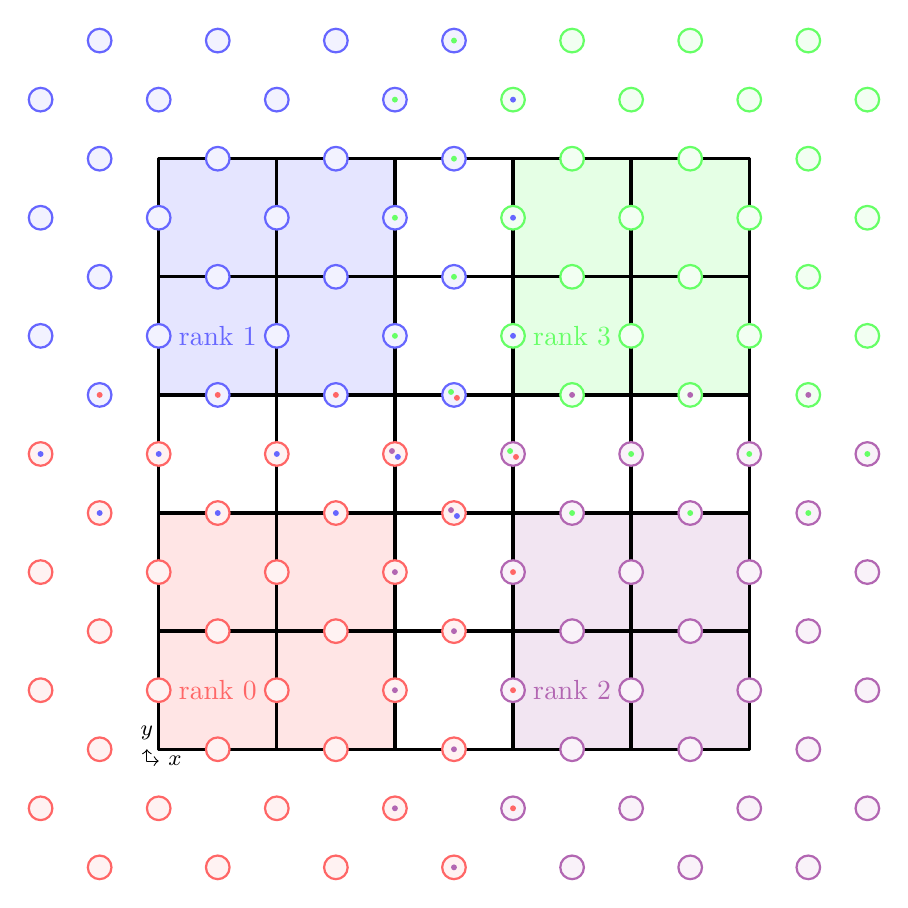
\begin{tikzpicture}[scale=1.5]
    \draw[black, line cap = round, ->] (-0.1,-0.1) -- (0,-0.1) node[color=black, anchor=west] {\footnotesize\(x\)};
    \draw[black, line cap = round, ->] (-0.1,-0.1) -- (-0.1,0) node[color=black, anchor=south] {\footnotesize\(y\)};
    

    \fill[fill=red!10] (0,0) rectangle (2,2) node[pos=0.25, color=red!60] {rank 0};
    \fill[fill=blue!10] (0,3) rectangle (2,5) node[pos=0.25, color=blue!60] {rank 1};
    \fill[fill=violet!10] (3,0) rectangle (5,2) node[pos=0.25, color=violet!60] {rank 2};
    \fill[fill=green!10] (3,3) rectangle (5,5) node[pos=0.25, color=green!60] {rank 3};

    % Horizontal lines
    \draw[black, very thick, line cap = round] (0,0) -- (5,0);
    \draw[black, very thick, line cap = round] (0,1) -- (5,1);
    \draw[black, very thick, line cap = round] (0,2) -- (5,2);
    \draw[black, very thick, line cap = round] (0,3) -- (5,3);
    \draw[black, very thick, line cap = round] (0,4) -- (5,4);
    \draw[black, very thick, line cap = round] (0,5) -- (5,5);

    % vertical lines
    \draw[black, very thick, line cap = round] (0,0) -- (0,5);
    \draw[black, very thick, line cap = round] (1,0) -- (1,5);
    \draw[black, very thick, line cap = round] (2,0) -- (2,5);
    \draw[black, very thick, line cap = round] (3,0) -- (3,5);
    \draw[black, very thick, line cap = round] (4,0) -- (4,5);
    \draw[black, very thick, line cap = round] (5,0) -- (5,5);


    \foreach \x in {-1,...,2}{
        \foreach \y in {-1,...,2}{
            \filldraw[color=red!60, fill=red!5, thick](\x,\y + 0.5) circle (0.1);
            \filldraw[color=red!60, fill=red!5, thick](\x + 0.5,\y) circle (0.1);
        }
    }


    \foreach \x in {-1,...,2}{
        \foreach \y in {3,...,5}{
            \filldraw[color=blue!60, fill=blue!5, thick](\x,\y + 0.5) circle (0.1);
            \filldraw[color=blue!60, fill=blue!5, thick](\x + 0.5,\y) circle (0.1);
        }
        \filldraw[color=blue!60, fill=blue!5, thick](\x + 0.5,6) circle (0.1);
    }

    \foreach \y in {-1,...,2}{
        \foreach \x in {3,...,5}{    
            \filldraw[color=violet!60, fill=violet!5, thick](\x,\y + 0.5) circle (0.1);
            \filldraw[color=violet!60, fill=violet!5, thick](\x + 0.5,\y) circle (0.1);
        }
        \filldraw[color=violet!60, fill=violet!5, thick](6,\y+0.5) circle (0.1);
    }

    \foreach \x in {3,...,5}{
        \foreach \y in {3,...,5}{
            \filldraw[color=green!60, fill=green!5, thick](\x,\y + 0.5) circle (0.1);
            \filldraw[color=green!60, fill=green!5, thick](\x + 0.5,\y) circle (0.1);
        }
        \filldraw[color=green!60, fill=green!5, thick](\x + 0.5,6) circle (0.1);
        \filldraw[color=green!60, fill=green!5, thick](6,\x + 0.5) circle (0.1);
    }


    \foreach \x in {-1,...,1}{
        \fill[fill=blue!60] (\x,2.5) circle (0.025);
        \fill[fill=blue!60] (\x+0.5,2) circle (0.025);

        \fill[fill=red!60] (\x+0.5,3) circle (0.025);
    }

    \fill[fill=green!60] (3.5,2) circle (0.025);
    \fill[fill=violet!60] (3.5,3) circle (0.025);
    \foreach \x in {4,...,5}{
        \fill[fill=green!60] (\x,2.5) circle (0.025);
        \fill[fill=green!60] (\x+0.5,2) circle (0.025);

        \fill[fill=violet!60] (\x+0.5,3) circle (0.025);
    }
    \fill[fill=green!60] (6,2.5) circle (0.025);

    \foreach \y in {-1,...,1}{
        \fill[fill=violet!60] (2.5,\y) circle (0.025);
        \fill[fill=violet!60] (2,\y+0.5) circle (0.025);
        
        \fill[fill=red!60] (3,\y+0.5) circle (0.025);
    }

    \fill[fill=green!60] (2,3.5) circle (0.025);
    \fill[fill=blue!60] (3,3.5) circle (0.025);
    \foreach \y in {4,...,5}{
        \fill[fill=green!60] (2.5,\y) circle (0.025);
        \fill[fill=green!60] (2,\y+0.5) circle (0.025);
        \fill[fill=blue!60] (3,\y+0.5) circle (0.025);
    }
    \fill[fill=green!60] (2.5,6) circle (0.025);



    \fill[fill=violet!60] (2-.025,2.5+.025) circle (0.025);
    \fill[fill=blue!60] (2+.025,2.5-.025) circle (0.025);

    \fill[fill=violet!60] (2.5-.025,2+.025) circle (0.025);
    \fill[fill=blue!60] (2.5+.025,2-.025) circle (0.025);

    \fill[fill=green!60] (3-.025,2.5+.025) circle (0.025);
    \fill[fill=red!60] (3+.025,2.5-.025) circle (0.025);

    \fill[fill=green!60] (2.5-.025,3+.025) circle (0.025);
    \fill[fill=red!60] (2.5+.025,3-.025) circle (0.025);

    % rank a DOFs
    %\filldraw[color=red!60, fill=red!5, thick](1,0.5) circle (0.1) node[color=black] {};
    %\filldraw[color=red!60, fill=red!5, thick](2,0.5) circle (0.1) node[color=black] {};
    %\filldraw[color=red!60, fill=red!5, thick](3,0.5) circle (0.1) node[color=black] {};
    %\filldraw[color=red!60, fill=red!5, thick](4,0.5) circle (0.1) node[color=black] {};
    %\filldraw[color=red!60, fill=red!5, thick](0.5,1) circle (0.1);
    %\fill[fill=blue!60] (0.5,1) circle (0.025);
    %\filldraw[color=red!60, fill=red!5, thick](1.5,1) circle (0.1) node[color=black] {};
    %\fill[fill=blue!60] (1.5,1) circle (0.025);
    %\filldraw[color=red!60, fill=red!5, thick](2.5,1) circle (0.1) node[color=black] {};
    %\fill[fill=blue!60] (2.5,1) circle (0.025);
    %\filldraw[color=red!60, fill=red!5, thick](3.5,1) circle (0.1) node[color=black] {};
    %\fill[fill=blue!60] (3.5,1) circle (0.025);
    %\filldraw[color=red!60, fill=red!5, thick](4.5,1) circle (0.1) node[color=black] {};
    %\fill[fill=blue!60] (4.5,1) circle (0.025);
    %\filldraw[color=red!60, fill=red!5, thick](1,1.5) circle (0.1) node[color=black] {};
    %\fill[fill=blue!60] (1,1.5) circle (0.025);
    %\filldraw[color=red!60, fill=red!5, thick](2,1.5) circle (0.1) node[color=black] {};
    %\fill[fill=blue!60] (2,1.5) circle (0.025);
    %\filldraw[color=red!60, fill=red!5, thick](3,1.5) circle (0.1) node[color=black] {};
    %\fill[fill=blue!60] (3,1.5) circle (0.025);
    %\filldraw[color=red!60, fill=red!5, thick](4,1.5) circle (0.1) node[color=black] {};
    %\fill[fill=blue!60] (4,1.5) circle (0.025);
%
%
    %% rank b DOFs
    %\filldraw[color=blue!60, fill=blue!5, thick](0.5,2) circle (0.1) node[color=black] {};
    %\fill[fill=red!60] (0.5,2) circle (0.025);
    %\filldraw[color=blue!60, fill=blue!5, thick](1.5,2) circle (0.1) node[color=black] {};
    %\fill[fill=red!60] (1.5,2) circle (0.025);
    %\filldraw[color=blue!60, fill=blue!5, thick](2.5,2) circle (0.1) node[color=black] {};
    %\fill[fill=red!60] (2.5,2) circle (0.025);
    %\filldraw[color=blue!60, fill=blue!5, thick](3.5,2) circle (0.1) node[color=black] {};
    %\fill[fill=red!60] (3.5,2) circle (0.025);
    %\filldraw[color=blue!60, fill=blue!5, thick](4.5,2) circle (0.1) node[color=black] {};
    %\fill[fill=red!60] (4.5,2) circle (0.025);
    %\filldraw[color=blue!60, fill=blue!5, thick](1,2.5) circle (0.1) node[color=black] {};
    %\filldraw[color=blue!60, fill=blue!5, thick](2,2.5) circle (0.1) node[color=black] {};
    %\filldraw[color=blue!60, fill=blue!5, thick](3,2.5) circle (0.1) node[color=black] {};
    %\filldraw[color=blue!60, fill=blue!5, thick](4,2.5) circle (0.1) node[color=black] {};

    


\end{tikzpicture}
    \caption{Example 2D \(6 \times 6\) domain decomposition into 4 ranks. The colored areas indicate that these elements are completely owned by that rank, the uncolored elements are shared between different ranks, i.e., multiple ranks have DOFs on them. The small colored dots inside of the degrees of freedom indicate that that rank has this DOF as part of their halo. Note that the \texttt{FEMVectors} expand one hyperplane of elements further out than the mesh (black grid), this also means that the element numbering for the global domain and the MPI subdomains have different origins. Also note that we do not make a halo exchange between rank 1 and rank 2.}
    \label{fig:domain_decomp2d}
\end{figure}

One of the main responsibilities of the \texttt{NedelecSpace} class with regards to the \texttt{FEMVector} is its creation. The \texttt{NedelecSpace} class provides a function, called \texttt{createFEMVector()}, which takes as input an MPI rank layout (calculated by \texttt{IPPL}) and returns a \texttt{FEMVector} for the MPI subdomain of the current rank with correct size and halo communication setup. We therefore need to discuss how the different boundaries with their halo cells are laid out. The layout provided by \texttt{IPPL} follows a vertex based approach, so it will provide a range of vertices which dictate the subdomains of each rank, this leads to some complication when having edge based DOFs, but a simple rule can be followed: a rank owns all the DOFs which are part of the elements that are engulfed by the vertex ranges of the layout. For example if the start of subdomain is marked by \((0,1)\) and the end by \((1,2)\), it would mean that this rank owns the elements \((0,1)\), \((1,1)\), \((0,2)\), and \((1,2)\). For a boundary where two MPI ranks meet, we have a hyperplane of elements which are owned by neither of the ranks, but both ranks have a DOF on opposing edges of the elements. There the rank for which this boundary is at the end of its domain will additionally own the DOFs on the edges connecting the two domains with the DOFs owned by the other rank in its halo. The rank for which the boundary is at the beginning of its domain will not get any additional DOFs, but will simply put all the ones the other rank owns into its halo. Naturally if the DOF is part of the halo of one rank (so part of the \texttt{recvIdxs}) it needs to be in the \texttt{sendIdxs} of the other rank. A visual representation of this for the 2D case can be seen in Figure \ref{fig:halo2d}, where a north south boundary is displayed, a west east would look identical just rotated \(90\) degrees clockwise. For 3D the same scheme is used, one simply adds a new dimension with everything else staying the same.\medskip

From these boundaries we can see that it appears as if we are growing one hyperplane of elements outwards, so if the layout dictates that the rank has a domain of size $\hat{m}_x \times \hat{m}_y \times \hat{m}_z$ elements it appears like we are actually interacting with a domain of size $\hat{m}_x + 2 \times \hat{m}_y + 2 \times \hat{m}_z + 2 = m_x \times m_y \times m_z$. Note that we are also adding one additional hyperplane of elements on the mesh domain boundary, to stay in line with this definition and to also allow for more complicated boundary conditions (like periodic) in the future. From this we then have that the \texttt{FEMvector} will store
\begin{align}
    \begin{cases}
    m_x(m_y-1) + m_y(m_x-1), &\text{for 2D} \\
    (m_z-1)(m_x(m_y-1) + m_y(m_x-1) + m_xm_y) + m_x(m_y-1) + m_y(m_x-1), &\text{for 3D}\\
    \end{cases}
\end{align}
elements. An example 2D decomposition for 4 ranks is given in Figure \ref{fig:domain_decomp2d}. Note that we have to pay special attention at points where multiple ranks meet, as it can get somewhat complicated trying to figure out which rank owns what. Another interesting fact is that for this case we would in theory have that rank 1 and rank 2 would exchange values over the diagonal, but in our implementation we are not doing such an exchange. Our test showed that this does not have an impact on the final result or the convergence of the algorithm. A similar thing is observed in 3D, where we do handle the diagonal exchange over edges, but not the diagonal exchange over corners, but again no impact on the error can be observed. We are not entirely sure why this happens and further research is required.\medskip

Now that we have established the DOFs which are stored by each \texttt{FEMVector} and how the boundary is handled the last thing we need to look at is the order in which these DOFs are stored inside of the \texttt{FEMVector} and related to that how we map between the global DOF numbering scheme (as displayed in Figure \ref{fig:glob_numbering}) and the entries in the \texttt{FEMVector}, i.e., given the global number of a DOF, what is its index in the \texttt{FEMVector}. For the ordering we follow the idea laid out in Section \ref{subsec:theory}, where we treat each MPI rank independently and do the numbering for its $m_x \times m_y \times m_z$ subdomain, note that when we are on the domain boundary the \texttt{FEMVector} is storing DOFs which are not part of the mesh, as the \texttt{FEMVector} is unaware of the mesh it will handle them like every other DOF. Then in order to translate between the global number of a DOF and its entry inside of the \texttt{FEMVector} we have to go over the element it belongs to, and there its local number (as displayed in Figure \ref{fig:ref_elements}). Suppose we have an element with a global position $\vec{p}$ in the mesh. This element will belong to a subdomain of a rank, where it will have a subdomain relative position of $\bar{\vec{p}}$. Then we can use Equations (\ref{eq:el2glob2d}) and (\ref{eq:el2glob3d}), replace $\vec{p}$ by $\bar{\vec{p}}$ and $n_x$, $n_y$, $n_z$ by $m_x$, $m_y$, $m_z$. These equations will then return the global DOF indices of all the DOFs related to this element, from them we then want to pick out the one which corresponds to our original DOF, which we do with the local shape function index, as we are working on the same element the local index of the original DOF will be the same as the one of DOF in the \texttt{FEMVector}. For example in Figure \ref{fig:domain_decomp2d} we want to get the \texttt{FEMVector} index of the DOF on the south edge (so local shape function index \(0\)) of the element with global position $\vec p = (3,1)$. This element lies in subdomain of rank 2 where it has a subdomain specific position of \(\bar{\vec{p}} = (1,2)\), note that here we are considering elements for which the \texttt{FEMVector} stores DOFs and because the \texttt{FEMVector} has DOFs outside of the mesh we have to include those elements (which are not part of the mesh) in our calculations, furthermore rank 2 has dimensions \(m_x \times m_y = 5\times 5\) and from this using Equation (\ref{eq:el2glob2d}) we figure out that the index of the DOF inside of the \texttt{FEMVector} is \(19\).\medskip

This might seem somewhat tedious to have to go over the element in order to translate indices, but in practice this does not lead to any problems, as for the assemble of the RHS, the evaluation of $A\vec v$, and the error metric calculations we are following an element based approach, where we loop over the elements and then for each of them do local calculations which we then translate to the global domain, therefore we always will be working with the shape functions of a given element, and it then is quite natural to both retrieve their global indices and their positions inside of the \texttt{FEMVector}.

\subsection{RHS}
\label{subsubsec:rhs}
%\begin{itemize}
%    \item Quickly write down variational formulation.
%    \item Quick overview on how this is done (loop over elements, for each,...)
%    \item Quick note about domain boundaries.
%\end{itemize}
The implementation of this is given by the function \texttt{evaluateLoadVector()}. In Galerkin FEM one generally transforms the problem in a linear system of equations \(A \vec \mu = \vec b\), here we will now discuss how we obtain the RHS \(\vec b\). The PDEs we are currently solving have a RHS which corresponds to a load term, which means that the $I$-th entry of the vector $\vec{b}$, of the linear system, is given by:
\begin{align}
    \vec{b}_I = \int_\Omega \vec{\beta}_I \cdot \vec{g}(\vec{x}) d\vec{x} \text{,}
\end{align}
where $\vec{\beta}_I$ is the basis function with global index $I$ and \(\vec g(\cdot)\) is the RHS function of the PDE we are solving. We implement this in standard FEM fashion using an element oriented assembling scheme, where we loop through all the elements, then for each of them calculate the local contribution of the local shape functions to the global basis indices, where we evaluate the integral using numerical quadrature. For a detailed description of the numerical quadrature used in \texttt{IPPL} refer to \cite{femIppl}. As we are currently only supporting zero Dirichlet boundaries in Nédélec FEM we skip all DOFs which are located on the boundary.\medskip

In theory the function $\vec{g}(\vec{x})$ will be provided by the PIC loop and how exactly this interface looks like is at this stage of the \texttt{IPPL} development not clear yet. Therefore we currently implemented it by passing a \texttt{FEMVector} which stores the values of $\vec g(\vec x)$ at the Nédélec DOF positions (center of edges) and we then do a very crude interpolation to the quadrature points using the distance between the edge centers and the quadrature nodes. One caveat that needs to be remembered here is that a \texttt{FEMVector} can never exist by itself and that it always needs a supporting structure. In this case of passing the RHS as a \texttt{FEMVector} it means we need to define what DOFs the \texttt{FEMVector} is storing, especially with regards to MPI ranks, and how they are ordered inside of it (here we are ignoring the halo, as we do not need to make any exchanges). In theory this is defined by the \texttt{NedelecSpace} class, but this leads to a problem, because the PIC loop would have to provide this vector and it does not know (and should not know) anything about the Nédélec space. This means that in the future some other way needs to be defined on how the RHS should be provided, one that is independent of the underlying FEM space being used. This is currently ongoing research in \texttt{IPPL}, also with regards to how interpolation between particles and mesh should be handled. In our implementation we are circumventing this problem by defining that the \texttt{FEMVector} that gets passed to the \texttt{evaluateLoadVector()} function needs to have a structure identical ont the one described is Section \ref{subsubsec:femvector}, except for any of the halo information (so simply the DOFs it stores and the order of this). We are able to do this as we are currently only solving standalone test cases without any PIC for which we manually defined the RHS. Therefore we can use our ``human'' knowledge to construct \texttt{FEMVector}s for these specific cases.


\subsection{Evaluate \(A\vec{v}\)}
\label{subsubsec:evaluateAx}
%\begin{itemize}
%    \item Quickly recap variational thing and that we get it from the solver.
%    \item Quick overview on how is done (similar to RHS)
%    \item Again note about boundary.
%\end{itemize}
In the previous section we saw how we obtain the RHS $\vec{b}$ of the system $A\vec{\mu} = \vec{b}$, now we discuss how the left hand side (LHS) is calculated. In theory one can explicitly construct the matrix $A$ and then solve the system directly, the problem with this approach is that for larger domain sizes the matrix $A$ can become very large making it unfeasible to store it inside of memory, especially on GPUs. For this reason we are taking a matrix-free approach in which we provide a functional that calculates the matrix vector product $A\vec{v}$, for some arbitrary $\vec{v}$, and combine this with an iterative solver, currently we use CG. Like this a much smaller memory footprint is achieved making the problem solvable even for large domains and higher orders. One part of this functional is the member function \texttt{evaluateAx()}\footnote{Note the somewhat different naming convention} that calculates the result of a multiplication between \(A\) and a vector \(\vec v\). \medskip

The entry $(I,J)$ for the global indices $I$ and $J$ of the matrix $A$ are given by:
\begin{align}
    A_{I,J} = \int_\Omega \mathcal{F}(\vec\beta_I, \vec\beta_J) d\vec{x}\text{,} \label{eq:varlhs}
\end{align}
where $\mathcal{F}(\vec\beta_I, \vec\beta_J)$ is related to the $F(\vec{u}(\vec{x}))$ of the \texttt{Solver} class through its variational formulation and it will be different for each type of problem that we want to solve. In order to obtain the product $A\vec{v} = \vec{s}$ we can say:
\begin{align}
\vec{s}_I = \sum_J A_{I,J} \vec{v}_J \label{eq:AxEval}
\end{align}
\medskip

In order to implement this in code we take a very similar approach to the calculation of the RHS. We loop through all the elements and then for each element \(K\) calculate the local element Matrix $\bar{A}$ which stores the contributions of the local shape functions of the element to the global matrix \(A\):
\begin{align}
    \bar{A}_{i,j} = \int_K \mathcal{F}(\vec\beta_i, \vec\beta_j) d\vec{x} \text{.}
\end{align}
Here the integral is solved using numerical quadrature and the $\mathcal{F}$ is provided to the \texttt{NedelecSpace} class by the \texttt{Solver} class through a functor that takes as input the basis function values and their curl at the quadrature points and returns the corresponding value of $\mathcal{F}(\cdot, \cdot)$. This approach allows for the solving of problems with arbitrary $F(\cdot)$, and in the future the parameters which are passed to the functional representation can be expanded to allow for the solving of problems which do not only rely on the basis function value and the curl. After the local element matrix $\bar{A}$ is constructed we use it to update $\vec{s}$ according to Equation (\ref{eq:AxEval}) where we need to map the local DOF indices $(i,j)$ to their global ones $(I,J)$ using the local to global mapping discussed previously. Like with the RHS the DOFs on the boundaries are skipped, due to their zero Dirichlet nature. After all this is done we should have an $\vec{s}$ which corresponds to the product $A\vec{v}$ and we can then take this entire function and pass it to the CG solver as an operator.


\subsection{Error metric}
\label{subsubsec:error_metric}
%\begin{itemize}
%    \item Say what sort of error we are solving for.
%    \item For this then get the coefficients of the DOFs.
%    \item Interpolate using basis functions to the Quadrature nodes.
%    \item Calc error and good is.
%\end{itemize}
In order to gauge the accuracy and correctness of our implementation we added an error metric namely the continuous L2 error, implemented by the function \texttt{computeError()}. The error that we are solving for is:
\begin{align}
    \epsilon = \int_\Omega |\vec{u}(\vec{x}) - \vec{u}_{sol}(\vec{x})|^2 d\vec{x}\text{,}
\end{align}
where $\vec{u}(\cdot)$ is our numerical solution and $\vec{u}_{sol}(\cdot)$ in an analytical solution. In true FEM fashion we do not compute this directly on a global level, but do it element wise, such that we have:
\begin{align}
    \epsilon = \sum_{K\in \text{elements}} \int_K |\vec{u}(\vec{x}) - \vec{u}_{sol}(\vec{x})|^2 d\vec{x}\text{.} \label{eq:errorLocalInt}
\end{align}
As we can see this would require us to have a functional representation of our solution $\vec{u}(\cdot)$, but in practice we have a vector $\vec{\mu}$ which corresponds to the basis function coefficients. In order to overcome this we utilize interpolation, specifically interpolation based on the basis functions. In order to get the value \(\vec{u}(\vec{x})\) for some \(\vec{x}\) inside of an element \(K\) we use:
\begin{align}
    \vec{u}(\vec{x}) = \sum_{i \in \text{local DOFs of }K} \mu_i \vec{\beta}_i(\vec{x})\text{,} \label{eq:interpolation}
\end{align}
where \(\mu_i\) is the basis function coefficient of the local shape function \(i\) and \(\vec{\beta}_i\) is the corresponding shape function. We then use numerical quadrature to evaluate the integral in Equation (\ref{eq:errorLocalInt}) and retrieve the final error. In standard FEM fashion we expect the error to decrease with second order when increasing the number of elements per dimension linearly.



\subsection{Solution reconstruction}

At the end of the day, after the problem has been solved, we need to pass the solution back to PIC, so we need a method for reconstructing the solution \(\vec u(\vec x)\) from the basis function coefficients \(\vec \mu\). Like with the RHS we also have here that the exact interface between PIC and FEM has not been designed yet. What we currently provide is a function called \texttt{reconstructToPoints()}, which takes as input a list of points inside of the mesh, stored in a \texttt{Kokkos::View}, and then reconstructs the function value of \(\vec u(\cdot)\) at these points and returns this as also as a \texttt{Kokkos::View}. In the future this might be used to directly retrieve the function value at the particle positions.\medskip

The implementation of this is rather straight forward and shares similarities to the error metric calculations. The general idea is that we loop through all the points, then for each point \(\vec w\) figure out to which element \(K\) it belongs too and then reconstruct the function value \(\vec u(\vec w)\) using the formula of Equation (\ref{eq:interpolation}), with \(\vec x\) replaced by \(\vec w\). Note that all this requires that the points passed to the function lie inside of the subdomain of the current MPI rank, which in turn means that every rank gets its unique set of positions. We think that this implementation makes more sense compared to one where a singular global set of positions is passed as each rank represents an individual unit that to a degree should be unaware of the global scheme and should generally only work on its subdomain.

\section{Solver}
%\begin{itemize}
%    \item Class to solve a problem of a specific type.
%    \item Provides the variational formulation of the lhs. Therefore have to create a new one for every problem we want solve.
%    \item Provide diagram showing workflow.
%    \item From initialisation creating the rhs thing to solve calling the CG.
%\end{itemize}
\begin{figure}[!h]
    \centering
    \begin{tikzpicture}[scale=1.5]
    \tikzumlset{fill class=red!5, draw=red!60, class width=20ex}
    \umlclass{ippl::Solver}{
        \# pcg\_algo\_m : ippl::CG\\
        ...
    }{
        + solve()\\
        + getL2Error()\\
        + reconstructToPoints()\\
        ...
    }

    \umlsimpleclass[y=3,x=-2]{ippl::Maxwell}
    \umlemptyclass[y=3,x=2]{ippl::FEMVector}


    \umlinherit{ippl::Solver}{ippl::FiniteElementSpace}
    
    \umlaggreg[mult1={\#lhsVector, \#rhsVector}]{ippl::Solver}{ippl::FEMVector}
\end{tikzpicture}
    \caption{UML Class diagram for the \texttt{Solver} class.}
    \label{fig:uml_solver}
\end{figure}

Finally we have the \texttt{Solver} class, displayed in Figure \ref{fig:uml_solver}, which contains the information for solving a problem of a specific type. This mainly boils down to providing a representation of the variational formulation of the LHS, corresponding to \(\mathcal{F}\), and storing the \texttt{FEMVector} representations of the RHS \(\vec{b}\) and the final solution vector \(\vec\mu\). Because the \(\mathcal{F}\) is unique for each problem that we are solving we have to create an individual class for each of these problem types. It also interacts with the Nédélec space to retrieve the RHS and the functor for the \(A\vec{v}\) multiplication, which it then passes to the CG solver. For example we implemented a class \texttt{FEMMaxwellDiffusionSolver} which solves a problem of the kind
\begin{align}
    &\nabla \times \nabla \times \vec{u}(\vec{x}) + \vec{u}(\vec{x}) = \vec{g}(\vec{x}) \text{ in } \Omega\\
    &\vec{u}(\vec{x}) \times \vec n =  \text{ on } \partial \Omega\text{,}
\end{align}
which we will discussed in more detail in Section \ref{sec:experiments} as part of our experiments.

Figure \ref{fig:gen_diag} already provided a simplified overview of how this works. More concrete we pass the RHS \(\vec{g}(\cdot)\) evaluated at the Nédélec DOFs to the constructor of the \texttt{Solver} class, which will assemble the RHS using the Nédélec space according to Section \ref{subsubsec:rhs} and store this inside of its \texttt{rhsVector} member. Then in order to solve the actual problem the function \texttt{solve()} is called which will first retrieve the functor for the \(A\vec{v}\) evaluation from the Nédélec space according to Section \ref{subsubsec:evaluateAx} with the help of its definition of \(\mathcal{F}\). After this both the RHS and the functor for \(A\vec{v}\) is passed to the CG solver which solves the entire problem and returns the basis function coefficients \(\vec{\mu}\) which are then stored in \texttt{lhsVector}, completing the solve routine.\medskip

After the problem has been solved we normally would pass the solution back to the PIC loop, but as this interface is not yet fully designed we currently do not do anything with the finished result and we simply store the basis function coefficients. But we also expose two functions \texttt{getL2Error()} and \texttt{reconstructToPoints()} which are wrappers around the \texttt{NedelecSpace::computeError()} and \texttt{NedelecSpace::reconstructToPoints()} functions of the Nédélec space which can be used during testing in order to gauge the correctness of the implementation.
\chapter{Results}
\label{sec:experiments}
%\begin{itemize}
%    \item In order to show correctness of implementation will solve a problem with two different RHS.
%    \item Explain the entire problem setup.
%    \item Create plot showcasing the convergence.
%    \item Show 2d plot of the solution.
%    \item Create some scaling study with strong and weak scaling for different problem sizes in both 2d and 3d.
%\end{itemize}

\section{Setup}
In this section we will test our implementation on one type of PDE, which is given by:
\begin{align}
    &\nabla \times \nabla \times \vec{u}(\vec{x}) + \vec{u}(\vec{x}) = \vec{g}(\vec{x}) \text{ in } \Omega \label{eq:strong}\\
    &\vec{u}(\vec{x}) \times \vec n =  \text{ on } \partial \Omega\text{,} \label{eq:boundary}
\end{align}
where \(\vec g (\vec x)\) is the source function, \(\vec u (\vec x)\) the solution, \(\vec n\) the domain normal (pointing outwards), and \(\Omega\) the domain with \(\partial \Omega\) being the boundary. For this PDE we define two different source functions \(\vec g(\vec x)\) and two different domains \(\Omega\). The first case, which we call ``Trigonometric'' has the following \(\vec g(\vec x)\) and \(\Omega\):
\begin{align}
    \vec{g}(\vec x) = 
    \begin{cases}
        \begin{bmatrix}
            (1+k^2)\sin(k y)\\ (1+k^2)\sin(k x)
        \end{bmatrix} & \text{ for 2D, with }\Omega=[1,3]^2\\
        \noalign{\vskip9pt}
        \begin{bmatrix}
            (1 + k^2)\sin(k y)\sin(k z) \\
            (1 + k^2)\sin(k x)\sin(k z) \\
            (1 + k^2)\sin(k x)\sin(k y)
        \end{bmatrix} & \text{ for 3D, with }\Omega=[1,3]^3\\
    \end{cases}\text{.}
\end{align}
The second case, which we call ``Polynomial'', has the following \(\vec g(\vec x)\) and \(\Omega\):
\begin{align}
    \vec{g}(\vec x) = 
    \begin{cases}
        \begin{bmatrix}
            2 - (y^2 - 1)\\ 2 - (x^2 - 1)
        \end{bmatrix}& \text{ for 2D, with }\Omega=[-1,1]^2\\
        \noalign{\vskip9pt}
        \begin{bmatrix}
            -2 (z^2 - 1) - 2 (y^2 - 1) + (y^2 - 1) (z^2 - 1) \\
            -2 (x^2 - 1) - 2 (z^2 - 1) + (x^2 - 1) (z^2 - 1) \\
            -2 (y^2 - 1) - 2 (x^2 - 1) + (x^2 - 1) (y^2 - 1)
        \end{bmatrix}& \text{ for 3D, with }\Omega=[-1,1]^3
    \end{cases}\text{.}
\end{align}
We then have that the exact solution \(\vec u (\vec x )\) for the Trigonometric problem is:
\begin{align}
    \vec{u}(\vec x) = 
    \begin{cases}
        \begin{bmatrix}
            \sin(k y)\\ \sin(k x)
        \end{bmatrix} & \text{ for 2D}\\
        \noalign{\vskip9pt}
        \begin{bmatrix}
            \sin(k y)\sin(k z) \\
            \sin(k x)\sin(k z) \\
            \sin(k x)\sin(k y)
        \end{bmatrix} & \text{ for 3D}\\
    \end{cases}\text{,}
\end{align}
and for the Polynomial one it is:
\begin{align}
    \vec{u}(\vec x) = 
    \begin{cases}
        \begin{bmatrix}
            - (y^2 - 1)\\ - (x^2 - 1)
        \end{bmatrix}& \text{ for 2D}\\
        \noalign{\vskip9pt}
        \begin{bmatrix}
            (y^2 - 1) (z^2 - 1) \\
            (x^2 - 1) (z^2 - 1) \\
            (x^2 - 1) (y^2 - 1)
        \end{bmatrix}& \text{ for 3D}
    \end{cases}\text{.}
\end{align}
\medskip

In order to solve the problem described by Equations (\ref{eq:strong}) and (\ref{eq:boundary}) using FEM we need to find its variational formulation. Luckily this is a very common type of problem and therefore this has already be done for us in \cite{maxwellBook}. The variational formulation is given by:
\begin{align}
    \int_{\Omega} \nabla \times \vec u(\vec x) \cdot \nabla \times \vec v(\vec x) d\vec x + \int_{\Omega} \vec u(\vec x) \cdot \vec v(\vec x) d\vec x = \int_{\Omega} \vec u(\vec x) \cdot \vec g(\vec x) d\vec x \text{, }\label{eq:varita}
\end{align}
where we enforce the zero dirichlet boundary by skipping DOFs located on the boundary. From this we now also can quite easily extract the \(\mathcal F (\cdot, \cdot)\) of Equation (\ref{eq:varlhs}):
\begin{align}
    \mathcal{F}\left(\vec u (\vec x), \vec v (\vec x)\right) = \nabla \times \vec u(\vec x) \cdot \nabla \times \vec v(\vec x) + \vec u(\vec x) \cdot \vec v(\vec x) \text{.}
\end{align}\medskip

During the element-based assembling scheme we are going to assemble the local matrices for the LHS and local parts of the vector for the RHS for every element in the mesh. In order to simplify calculations we are not going to work on the actual elements of the mesh, but rather on the reference element. In Section \ref{subsec:theory} we already introduced the transformations required, our problem transforms into:
\begin{align}
    & A_{i,j} = \int_{K} \nabla \times \vec \beta_i \cdot \nabla \times \beta_j d\vec x  + \int_{K} \vec \beta_i \cdot \vec \beta_j d\vec x = \int_{\hat K} J^{-T}(\nabla \times \hat{\vec\beta}_i) \cdot J^{-T} (\nabla \times \hat{\vec\beta}_j) d\vec x + \int_{\hat K} \hat{\vec\beta}_i \cdot \hat{\vec\beta}_j d\vec x \text{,}\\
    & s_{i} = \int_{K} \vec \beta_i \cdot \vec g(\vec x) d\vec x = \int_{\hat K} \hat{\vec\beta}_i \cdot \vec g(\vec x) d\vec x \text{,}
\end{align}
where $J^{-T}$ is the inverse transpose Jacobian of the affine transformation between the reference and the actual element.\medskip


\section{Correctness}
\begin{figure}
    \centering
    \begin{subfigure}{0.49\textwidth}
        \centering
        \includegraphics[width=\linewidth]{figures/experiments/convergence_trig.pdf}
        \caption{Trigonometric case.}
    \end{subfigure}
    \begin{subfigure}{0.49\textwidth}
        \centering
        \includegraphics[width=\linewidth]{figures/experiments/convergence_poly.pdf}
        \caption{Polynomial case.}
    \end{subfigure}
    \caption{L2 error convergences for the different problems. As we can see, perfect order 2 convergence is achieved.}
    \label{fig:convergence}
\end{figure}
\begin{table}
    \centering
    \begin{subtable}{\textwidth}
        \centering
        \begin{Large}
            Trigonometric problem
        \end{Large}
        \begin{small}
            \begin{tabular}{ccc@{\hskip 1cm}cc}
                \toprule
                & \multicolumn{2}{c}{2D\hphantom{asdf}} & \multicolumn{2}{c}{3D} \\
                Num nodes & L2 Error & Iterations & L2 Error & Iterations \\
                \cmidrule(lr{1cm}){2-3}\cmidrule(r){4-5}
                \( 16\)   &  \(5.125\cdot 10^{-2}\)  & \(  13\)  &  \(1.168\cdot 10^{-1}\) & \(   5\) \\
                \( 22\)   &  \(2.626\cdot 10^{-2}\)  & \(  19\)  &  \(6.013\cdot 10^{-2}\) & \(   8\) \\
                \( 31\)   &  \(1.290\cdot 10^{-2}\)  & \(  29\)  &  \(2.961\cdot 10^{-2}\) & \(  15\) \\
                \( 43\)   &  \(6.586\cdot 10^{-3}\)  & \(  42\)  &  \(1.514\cdot 10^{-2}\) & \(  22\) \\
                \( 60\)   &  \(3.339\cdot 10^{-3}\)  & \(  61\)  &  \(7.682\cdot 10^{-3}\) & \(  35\) \\
                \( 84\)   &  \(1.688\cdot 10^{-3}\)  & \(  89\)  &  \(3.884\cdot 10^{-3}\) & \(  54\) \\
                \(118\)   &  \(8.495\cdot 10^{-4}\)  & \( 165\)  &  \(1.955\cdot 10^{-3}\) & \(  93\) \\
                \(166\)   &  \(4.272\cdot 10^{-4}\)  & \( 248\)  &  \(9.833\cdot 10^{-4}\) & \( 233\) \\
                \(234\)   &  \(2.142\cdot 10^{-4}\)  & \( 335\)  &  \(4.932\cdot 10^{-4}\) & \( 343\) \\
                \(330\)   &  \(1.074\cdot 10^{-4}\)  & \(1026\)  &  \(2.474\cdot 10^{-4}\) & \( 994\) \\
                \(466\)   &  \(5.379\cdot 10^{-5}\)  & \(1609\)  &  \(1.238\cdot 10^{-4}\) & \(2321\) \\
                \(659\)   &  \(2.686\cdot 10^{-5}\)  & \(2963\)  &  \(6.184\cdot 10^{-5}\) & \(3883\) \\
                \(931\)   &  \(1.345\cdot 10^{-5}\)  & \(4261\)  &  \(3.096\cdot 10^{-5}\) & \(6185\) \\
                \bottomrule
            \end{tabular}
        \end{small}
    \end{subtable}
    \vskip 1cm
    \begin{subtable}{\textwidth}
        \centering
        \begin{Large}
            Polynomial problem
        \end{Large}
        \begin{small}
            \begin{tabular}{ccc@{\hskip 1cm}cc}
                \toprule
                & \multicolumn{2}{c}{2D\hphantom{asdf}} & \multicolumn{2}{c}{3D} \\
                Num nodes & L2 Error & Iterations & L2 Error & Iterations \\
                \cmidrule(lr{1cm}){2-3}\cmidrule(r){4-5}
                \( 16\)   &  \(8.824\cdot 10^{-3}\)  & \(   7\)  &  \(2.293\cdot 10^{-2}\) & \(  23\) \\
                \( 22\)   &  \(4.502\cdot 10^{-3}\)  & \(  12\)  &  \(1.171\cdot 10^{-2}\) & \(  36\) \\
                \( 31\)   &  \(2.206\cdot 10^{-3}\)  & \(  19\)  &  \(5.741\cdot 10^{-3}\) & \(  56\) \\
                \( 43\)   &  \(1.125\cdot 10^{-3}\)  & \(  29\)  &  \(2.930\cdot 10^{-3}\) & \(  81\) \\
                \( 60\)   &  \(5.703\cdot 10^{-4}\)  & \(  43\)  &  \(1.485\cdot 10^{-3}\) & \( 119\) \\
                \( 84\)   &  \(2.882\cdot 10^{-4}\)  & \(  62\)  &  \(7.503\cdot 10^{-4}\) & \( 170\) \\
                \(118\)   &  \(1.450\cdot 10^{-4}\)  & \(  90\)  &  \(3.776\cdot 10^{-4}\) & \( 267\) \\
                \(166\)   &  \(7.291\cdot 10^{-5}\)  & \( 185\)  &  \(1.899\cdot 10^{-4}\) & \( 382\) \\
                \(234\)   &  \(3.657\cdot 10^{-5}\)  & \( 178\)  &  \(9.522\cdot 10^{-5}\) & \( 640\) \\
                \(330\)   &  \(1.834\cdot 10^{-5}\)  & \( 483\)  &  \(4.776\cdot 10^{-5}\) & \(1039\) \\
                \(466\)   &  \(9.181\cdot 10^{-6}\)  & \(1113\)  &  \(2.391\cdot 10^{-5}\) & \(2086\) \\
                \(659\)   &  \(4.585\cdot 10^{-6}\)  & \(2220\)  &  \(1.194\cdot 10^{-5}\) & \(3592\) \\
                \(931\)   &  \(2.295\cdot 10^{-6}\)  & \(3600\)  &  \(5.977\cdot 10^{-6}\) & \(5804\) \\
                \bottomrule
            \end{tabular}
        \end{small}
    \end{subtable}
    \caption{Tables with exact values of the convergence studies. Additionally the number of CG iterations is also given.}
    \label{tab:convergence}
\end{table}
In order to gauge the correctness of the implementation a convergence study is done. To this extend the problems are solved multiple times while increasing the mesh resolution, for each case the L2 error as described in Section \ref{subsubsec:error_metric} is calculated and the result is plotted. For these experiments we went with number of nodes per dimension in the range of \(16\) to \(931\), a Gauss Jacobi quadrature using 5 nodes per dimension for the numerical quadrature is used, and the linear system is solved using a non-preconditioned conjugate gradient algorithm with tolerance set to \(10^{-13}\) and maximum number of iterations set to \(10000\). The plots resulting from this can be seen in Figure \ref{fig:convergence} with exact values given in Table \ref{tab:convergence}. From theory we would expect the error to converge with a rate of $\Theta(n^{-2})$ where $n$ is the number of vertices per dimension. As we can see in the plots we have this convergence, as expected.\medskip


\section{Scaling Analysis}
\begin{figure}
    \centering
    \begin{subfigure}{0.49\textwidth}
        \centering
        \includegraphics[width=\linewidth]{figures/experiments/scaling_strong_2d.pdf}
        \caption{2D case}
        \label{fig:scalingStrong2D}
    \end{subfigure}
    \begin{subfigure}{0.49\textwidth}
        \centering
        \includegraphics[width=\linewidth]{figures/experiments/scaling_strong_3d.pdf}
        \caption{3D case}
        \label{fig:scalingStrong3D}
    \end{subfigure}
    \caption{Strong scaling of the implementation. All runs where repeated 10 times with an additional warm-up run, mean and confidence intervals are plotted.}
    \label{fig:scalingStrong}
\end{figure}
\begin{figure}
    \centering
    \begin{subfigure}{0.49\textwidth}
        \centering
        \includegraphics[width=\linewidth]{figures/experiments/scaling_weak_2d.pdf}
        \caption{2D case}
        \label{fig:scalingWeak2D}
    \end{subfigure}
    \begin{subfigure}{0.49\textwidth}
        \centering
        \includegraphics[width=\linewidth]{figures/experiments/scaling_weak_3d.pdf}
        \caption{3D case}
        \label{fig:scalingWeak3D}
    \end{subfigure}
    \caption{Weak scaling of the implementation. All runs where repeated 10 times with an additional warm-up run, mean and confidence intervals are plotted.}
    \label{fig:scalingWeak}
\end{figure}

\begin{table}
    \centering
    \begin{subtable}{0.49\textwidth}
        \begin{center}
\begin{tabular}{cc}
\toprule
\multicolumn{1}{c}{Num nodes}&\multicolumn{1}{c}{Time [s]}\tabularnewline
\midrule
$~4096$&$~0.6828832287$\tabularnewline
$~8192$&$~2.4991507782$\tabularnewline
$16384$&$11.3711869943$\tabularnewline
\bottomrule
\end{tabular}\end{center}

        \caption{2D case}
        \label{tab:time2d}
    \end{subtable}
    \begin{subtable}{0.49\textwidth}
        \begin{center}
\begin{tabular}{cc}
\toprule
\multicolumn{1}{c}{Num nodes}&\multicolumn{1}{c}{Time [s]}\tabularnewline
\midrule
$128$&$~0.7920425589$\tabularnewline
$256$&$~5.7699309643$\tabularnewline
$512$&$45.0464857090$\tabularnewline
\bottomrule
\end{tabular}\end{center}

        \caption{3D case}
        \label{tab:time3d}
    \end{subtable}
    \caption{Runtimes for for the scaling experiments in the case of a singular rank. The mean over the runs is calculated. Note that here in the case of a singular rank it does not matter if we consider the strong or the weak scaling case.}
\end{table}


We also perform a small scaling study of our implementation in the form of a strong and weak scaling analysis. The hardware setup we used for the runs consists of a two node setup, each equipped with a dual socket \(128\) core \texttt{AMD EPYC 7773X} and \(1\)TB of memory, and four \texttt{NVIDIA A100}s with \(80\)GB of memory each. For the network a \(200\)Gb/s Infiniband connection is used, and the MPI is a cuda aware \texttt{OpenMPI 5.0.3} instance, the operating system is \texttt{Rocky Linux 9.4}. For the runs we only consider the Polynomial case, as the performance between the two cases should be the same. It was configured identically to the previous section, with the exception that for both strong and weak scaling the maximum number of CG iterations are set to \(100\) and the tolerance is set to a negative value, like this we have that the number of CG iterations stays constant over the different domain sizes and therefore the work required is directly related to the domain size (which is critical for the weak scaling). All runs where repeated \(10\) times with an additional warm-up run for which then mean and confidence intervals are calculated. For strong scaling in 2D we went with problem sizes of \(4096^2\), \(8192^2\), and \(16384^2\) which where run with \(1\), \(2\), \(4\), and \(8\) ranks (where only for the case of \(8\) ranks we move to two nodes), this can be seen in Figure \ref{fig:scalingStrong2D}, with base runtimes in Table \ref{tab:time2d}. For the strong scaling in 3D we went with problem sizes of \(128^3\), \(256^3\), and \(512^3\) with same range of ranks, this can be seen in Figure \ref{fig:scalingStrong3D}, with base runtimes in Table \ref{tab:time3d}. For the weak scaling in 2D the base sizes where \(4096^2\), \(8192^2\), and \(16384^2\), they where scaled with the number of ranks \(p\) with the formula \(\sqrt{p}\:n_{base}\), where \(n_{base}\) is one of the base sizes. The number of processes was again in the range of \(1\) to \(8\), the results of this can be seen in Figure \ref{fig:scalingWeak2D}, with the base runtimes given in Table \ref{tab:time2d}. For the weak scaling in 3D the base sizes where \(128^3\), \(256^3\), and \(512^3\), the update formula for more processes is given by \(\sqrt[3]{p}\:n_{base}\), with same number of processes as in all other experiments, this can be seen in Figure \ref{fig:scalingWeak3D}, with base runtimes given in Table \ref{tab:time3d}. Generally for all the experiments here we were not able to go to any larger problem sizes due to having not enough memory on the GPUs.\medskip

From the plots we get a somewhat mixed result, we can unsurprisingly see that for smaller problem sizes both the strong and weak scaling perform bad, for example in the strong scaling 3D case we have that for a problem size of \(128\) no more scaling can be seen for more than 2 ranks. If we move to larger problem sizes the scaling tends to get better, but they are still not satisfactory. For example for the largest problem size in 3D we already drop to around \(90\%\) parallel efficiency at \(8\) ranks, for 2D we are able to hold ourselves better and remain at \(94\%\). For the speed-up in both 2D and 3D for the largest problem size and \(8\) ranks we already drop to \(72\%\) of the optimal speed-up. And all this is for the case of only \(8\) GPUs, in theory we would like to go to much more. So in theory the larger the problem size the better, but here we then start to run into a different issue: memory. We cannot go to larger problem sizes, because they simply stop fitting into GPU memory. For example in the 3D case with problem size of \(1024^3\) we have that already only the representation of the RHS \(\vec g(\vec x)\) at the DOFs using double precision requires around \(77\)GB of memory, which barely fits into a GPU. So we have the problem of needing to parallelize because we do not have enough memory, but at the point at which we have to parallelize the program does not yet scale well and we would actually like to go larger. Trying to decrease the memory footprint would be rather difficult, as at one point we have to store the \texttt{FEMVectors} on device. One could maybe try to do something with regard to storing the entire data in CPU and then only moving it part-wise to GPU, this would help with the amount of memory that is needed on device, but would introduce more complexity and overhead every time data needs to be copied to device and back. Another approach would be to try to decrease the overhead generated by the parallelization, which in turn would lead to better scaling behaviour for all problem sizes and we therefore do not run into the issue of the scaling behaviour being bad for the sizes at which we parallelize. We therefore can see that still some work could be done in this area.
\chapter{Conclusion}
\label{chapter:conclusion}

In this work we presented an implementation of the Langevin collision operator via a Particle-in-Cell
scheme for modeling the Vlasov-Poisson-Fokker-Planck equation.
We explored multiple methods for solving the electrostatic and Rosenbluth potentials by comparing
their performance to analytical test cases.
Additionally, we demonstrated 2\textsuperscript{nd} order algebraic error convergence for both the dynamical friction
and diffusion term.

Subsequently, we applied the solver to the challenging problem of simulating the disorder induced
heating process (\gls{dih}) in an initially cold sphere.
Analyzing the impact of the coefficients on the normalized emittance, we found the friction
coefficient to be too small to cause any effect.
A possible explanation is that the \gls{dih} problem starts off from
an unphysical zero velocity initial condition.
We showed that the diffusion matrices during the first few plasma periods tend to be negative
definite when close to the simulation boundary. This property inhibits the Euler-Maruyama time
integration method as it makes use of the matrices Cholesky decomposition.
Further investigation showed that the frequency at which such negative definite matrices occur rapidly
decreases after the off-diagonal elements start to show an oscillatory behavior.
This indicates that there is some warm-up time in which assumptions on the collisional operator could
be violated, leading to these unphysical diffusion matrices.

During our investigations of appropriate numerical operators for the Rosenbluth potentials,
we developed a tool that enables the composition of user-defined operators into a single
callable instance that is generated at compile time.
\newpage
\section{Outlook}

The investigation on the Langevin collision operator gave rise to many unexpected and interesting questions which
could be explored in a potential continuation of this project.

We divide this section into suggestions serving two differing purposes:

\begin{enumerate}
    \item Further investigation on the collision operator when applied to the \gls{dih} problem.
    \item Possible algorithmic and general performance improvements.
\end{enumerate}

We suggest a continuation of the investigation on the apparent negative definiteness of the
diffusion matrices in the early stages of the \gls{dih} simulation. Especially, we think is beneficial to
better understand the origin of the noise that impacts the off-diagonal entries. Also, it could help
to inspect how the eigenvalues are distributed between the matrices.
As an intermediate solution, one could use a diagonal restriction of the afflicted matrices, making them
factorizable. The \gls{ldlt} decomposition we currently use would allow this to be implemented without
much overhead. However, we point out that one should be aware of and investigate possible negative
impacts this linearization brings along.

Another direction of research could be, to better understand how the interplay between mesh
spacing and time step influences the collisional coefficients' values. This has partly been explored
by Stoel \cite{stoel} on another test case, though we expect it to be of even higher importance in
the \gls{dih} problem due to the peculiar initial conditions causing a discontinuity at the origin.
We suggest exploring this with methods akin to the one used by Adam
\cite{subcyclingAdam1982}, also known as subcycling, during the early stages of the simulation.
Similarly as the number of macro-particles per cell is low for most of the velocity domain it would be
worthwile investigating how increasing this number reduces the observed error in the collisional
coefficients.

We have shown the correctness of our collisional operator on analytical test cases.
Thus, we suggest testing it on a simpler physical test case to examine if we
encounter similar issues as with the \gls{dih} problem or not.
As an example a stationary initial velocity distribution (i.e. Maxwellian) could be used.
This would also allow investigating the energy dissipation introduced by the Euler-Maruyama integrator.

This report has been a case study of the applicability of a collisional operator to the \gls{dih} problem.
Our main focus did not lie on implementing a highly optimized and efficient solver before we could
show its correctness. Nevertheless, during the development process we have found many ways how one
could optimize it.
The current implementation of the solver supports shared-memory parallelism with \gls{openmp} and
\gls{simd} parallelism via single GPU execution.
Distributed memory parallelism (via \gls{mpi}) is currently not supported due to the domain
decomposition being defined solely by the particle distribution on the spatial grid.
One could implement the concept of super-cells introduced by Qiang \cite{qiang2000self} which uses
separate velocity grids for each \gls{mpi} rank to circumvent these limitations.
Another potential performance improvement concerns the computation of the two collisional terms.
It could be carried out completely asynchronously on the GPU via the CUDA streams concept,
as their computation is independent up to the point where the collisional coefficients are used
to update the particle velocities.




\bibliography{report}

\end{document}